\documentclass[11pt,a4paper]{article}
\usepackage[margin=22mm]{geometry}
\usepackage[T1]{fontenc}
\usepackage{lmodern}
\usepackage{amsmath}
\usepackage{booktabs}
\usepackage{tabularx}
\usepackage{array}
\usepackage{float}
\usepackage{graphicx}
\usepackage{pdfpages}
\usepackage{hyperref}
\usepackage{caption}
\hypersetup{colorlinks=true,linkcolor=blue,urlcolor=blue,citecolor=blue}
\graphicspath{{SupplementaryData/figures/}}

\title{Supplementary Information\\[0.4em]
\large Sensitivity of Fuzzy-PSO Inertia Control to Linguistic Granularity and Rule-Base Structure}
\author{}
\date{15 October 2026}

\begin{document}
\maketitle
\tableofcontents
\clearpage

\section{Fuzzy-controller configuration space}

The main article shows representative panels. This section documents the full set of evaluated membership partitions, rule patterns, and induced control surfaces for all four granularities, $n\in\{3,5,7,9\}$. The input and output partition families are I1 and O1 throughout.

\subsection{Diversity input partition}
\begin{figure}[H]\centering
  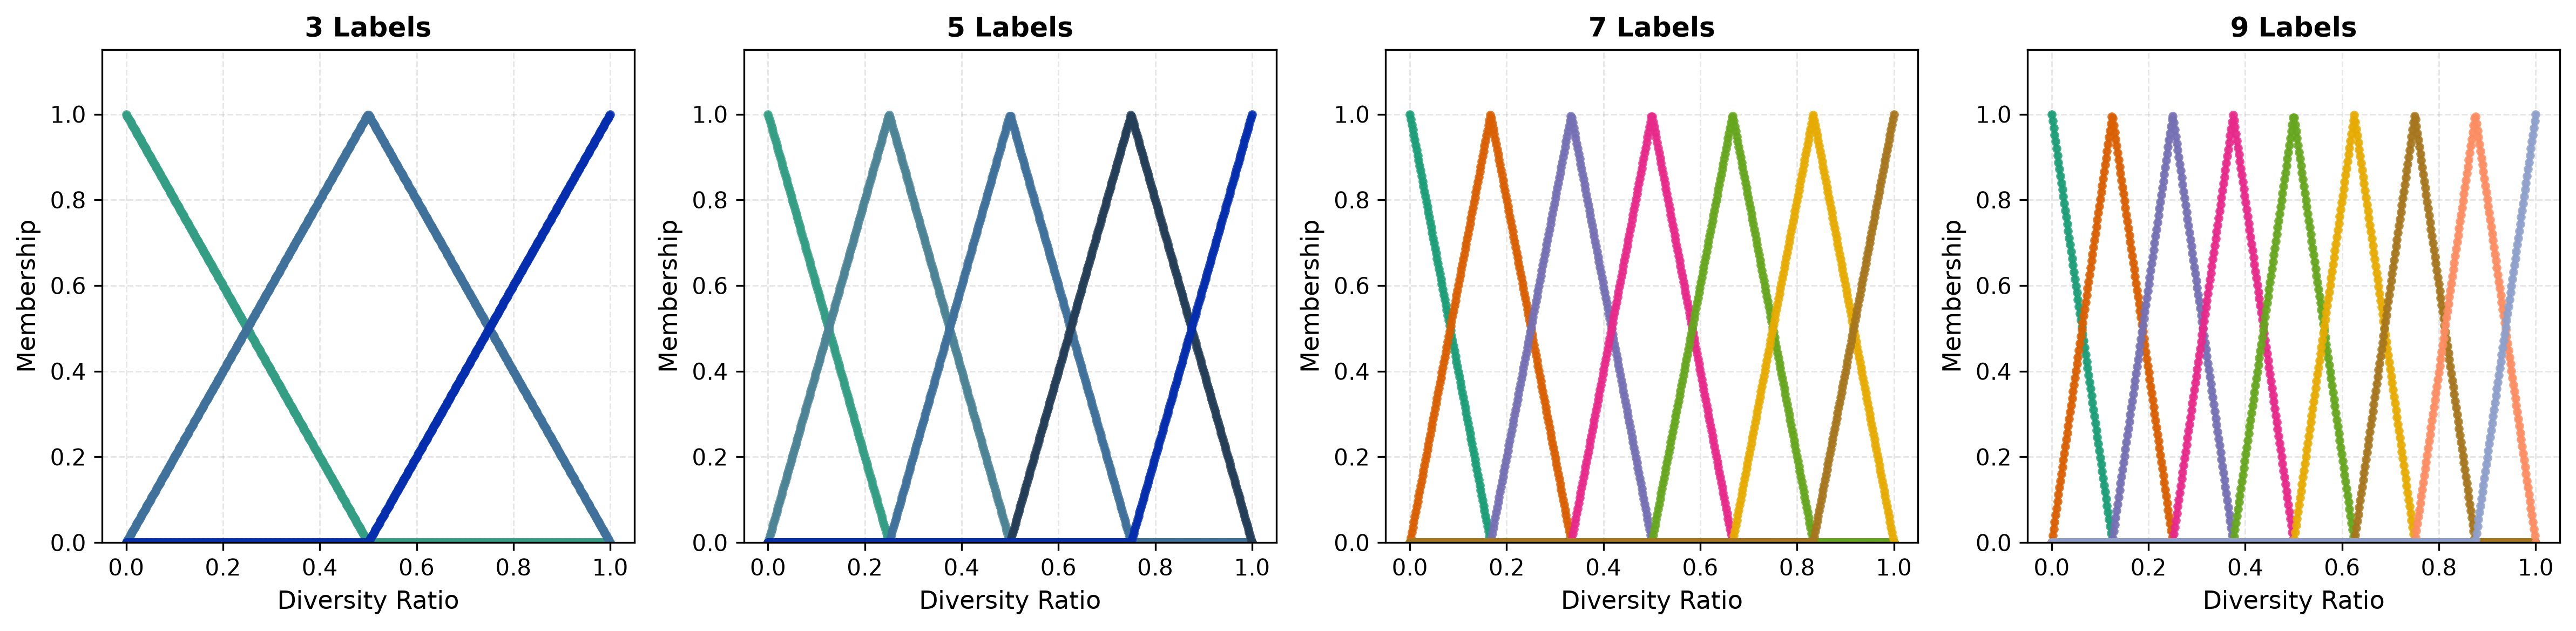
\includegraphics[width=\textwidth,height=0.72\textheight,keepaspectratio]{06_input_diversity_mf_panel_I1.png}
  \captionof{figure}{Diversity-input membership functions for all evaluated granularities.}
\end{figure}

\subsection{Progress input partition}
\begin{figure}[H]\centering
  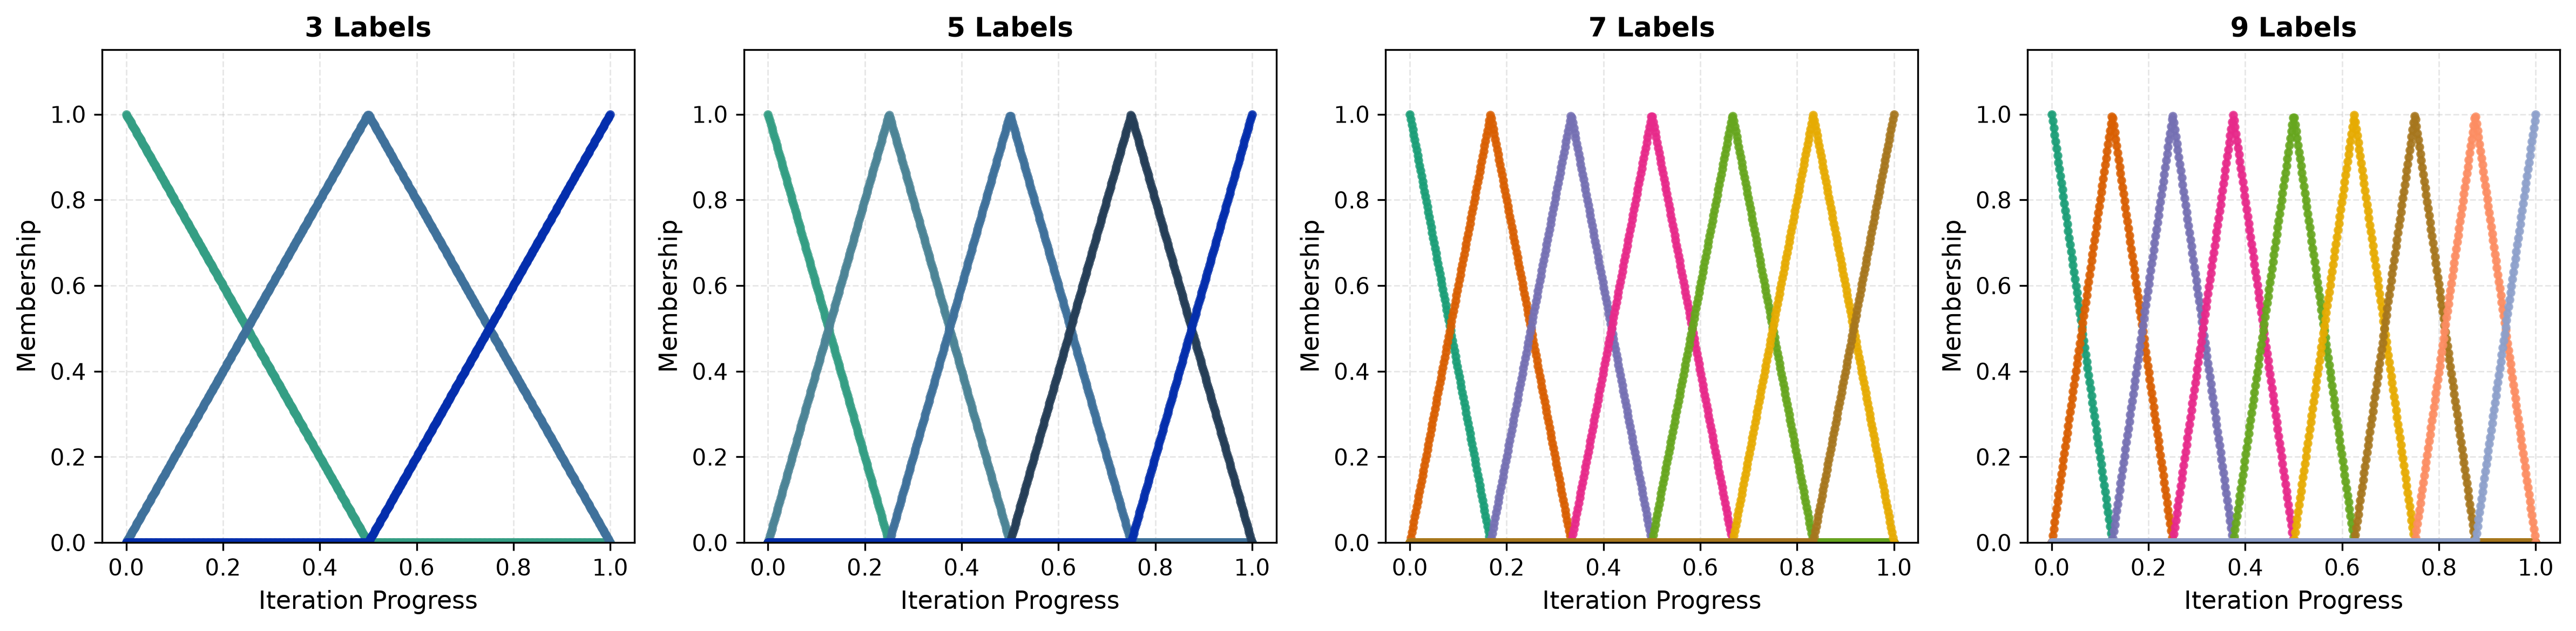
\includegraphics[width=\textwidth,height=0.72\textheight,keepaspectratio]{07_input_progress_mf_panel_I1.png}
  \captionof{figure}{Progress-input membership functions for all evaluated granularities.}
\end{figure}

\subsection{Inertia-weight output partition}
\begin{figure}[H]\centering
  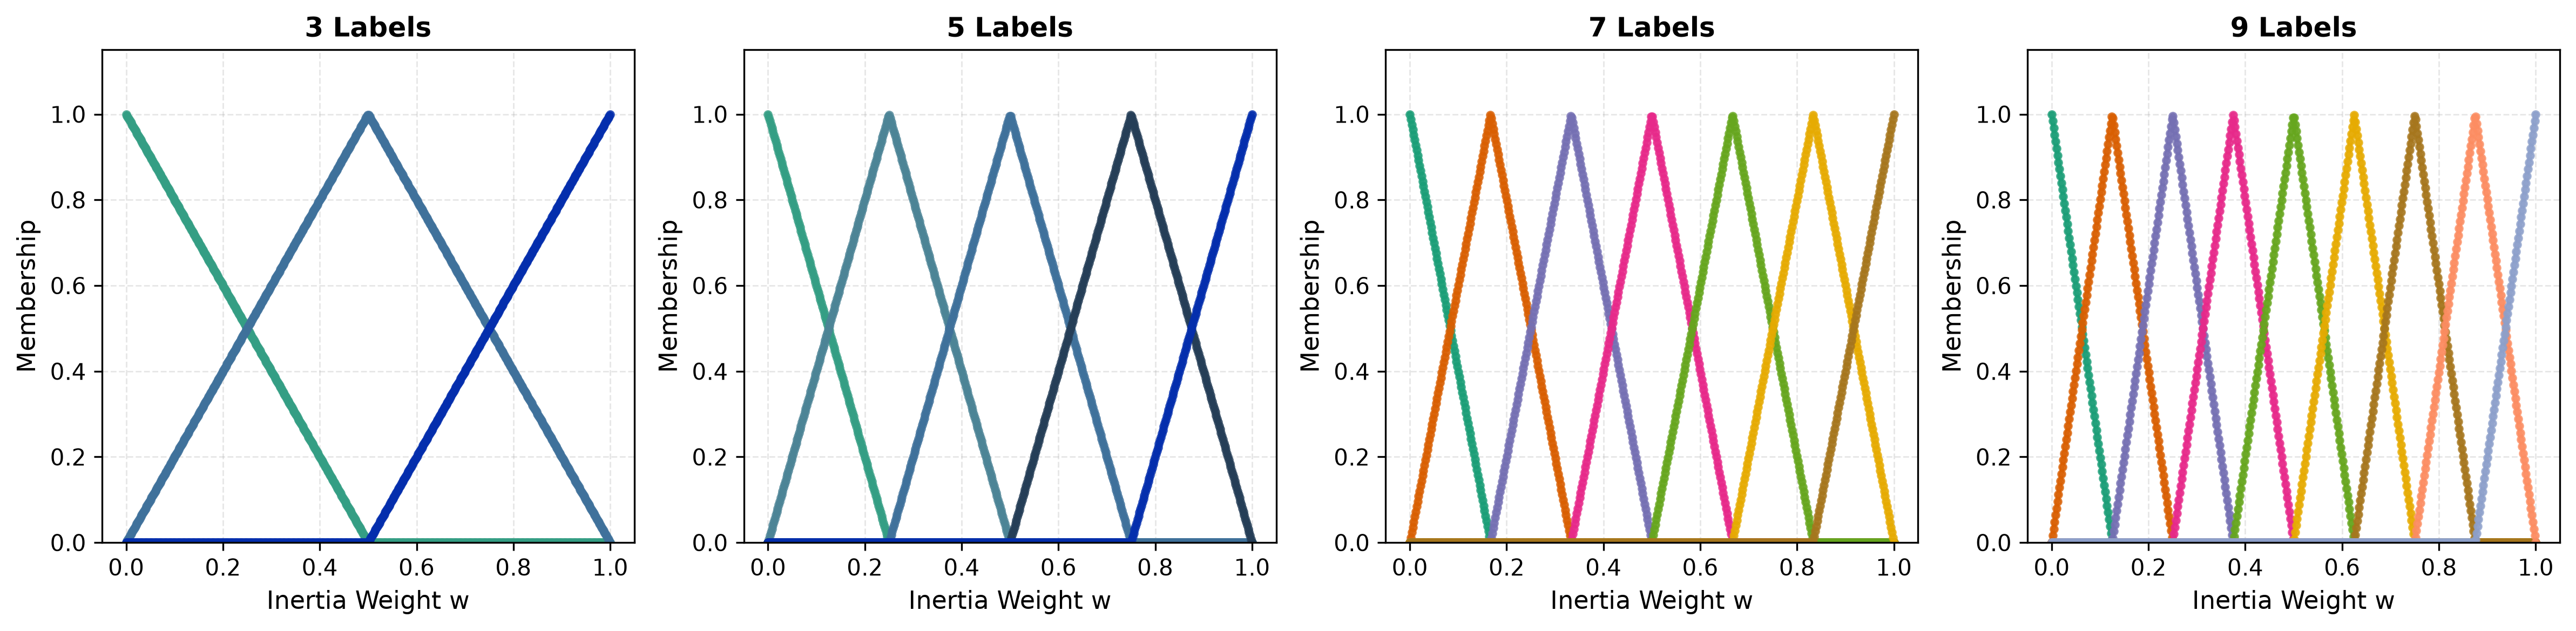
\includegraphics[width=\textwidth,height=0.72\textheight,keepaspectratio]{08_output_w_mf_panel.png}
  \captionof{figure}{Output membership functions for the inertia weight, $w\in[0.1,0.9]$, for all evaluated granularities.}
\end{figure}

\subsection{Rule-base matrices}
Each panel contains R1--R8 for the indicated granularity. Cell abbreviations and the shared colour scale are defined in the corresponding figure.
\begin{figure}[H]\centering
  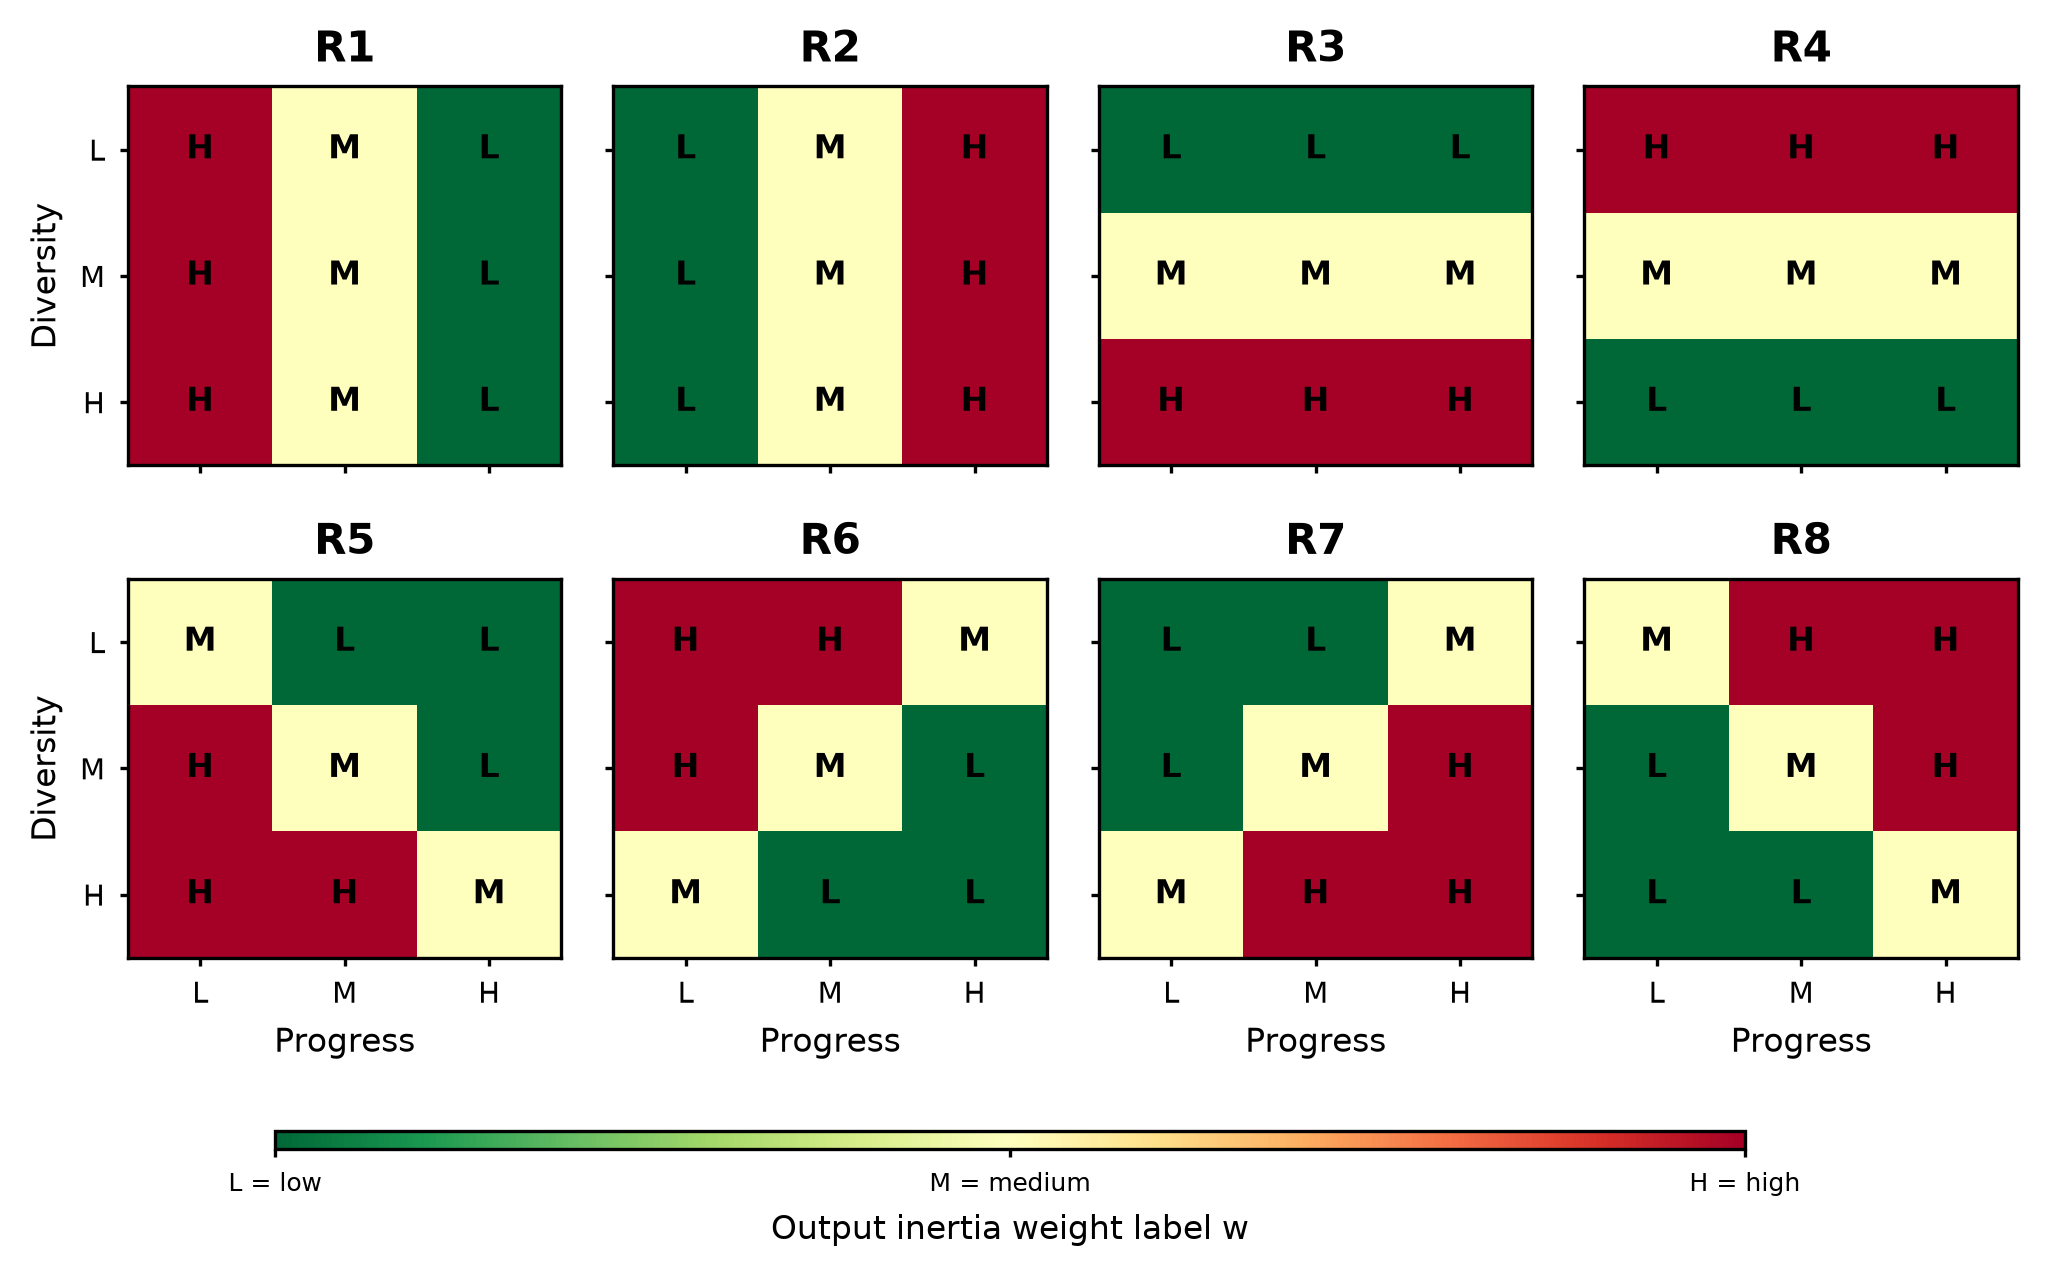
\includegraphics[width=\textwidth,height=0.82\textheight,keepaspectratio]{04_fuzzy_rules_panel_3labels.png}
  \captionof{figure}{Rule-base matrix panel for $n=3$.}
\end{figure}
\begin{figure}[H]\centering
  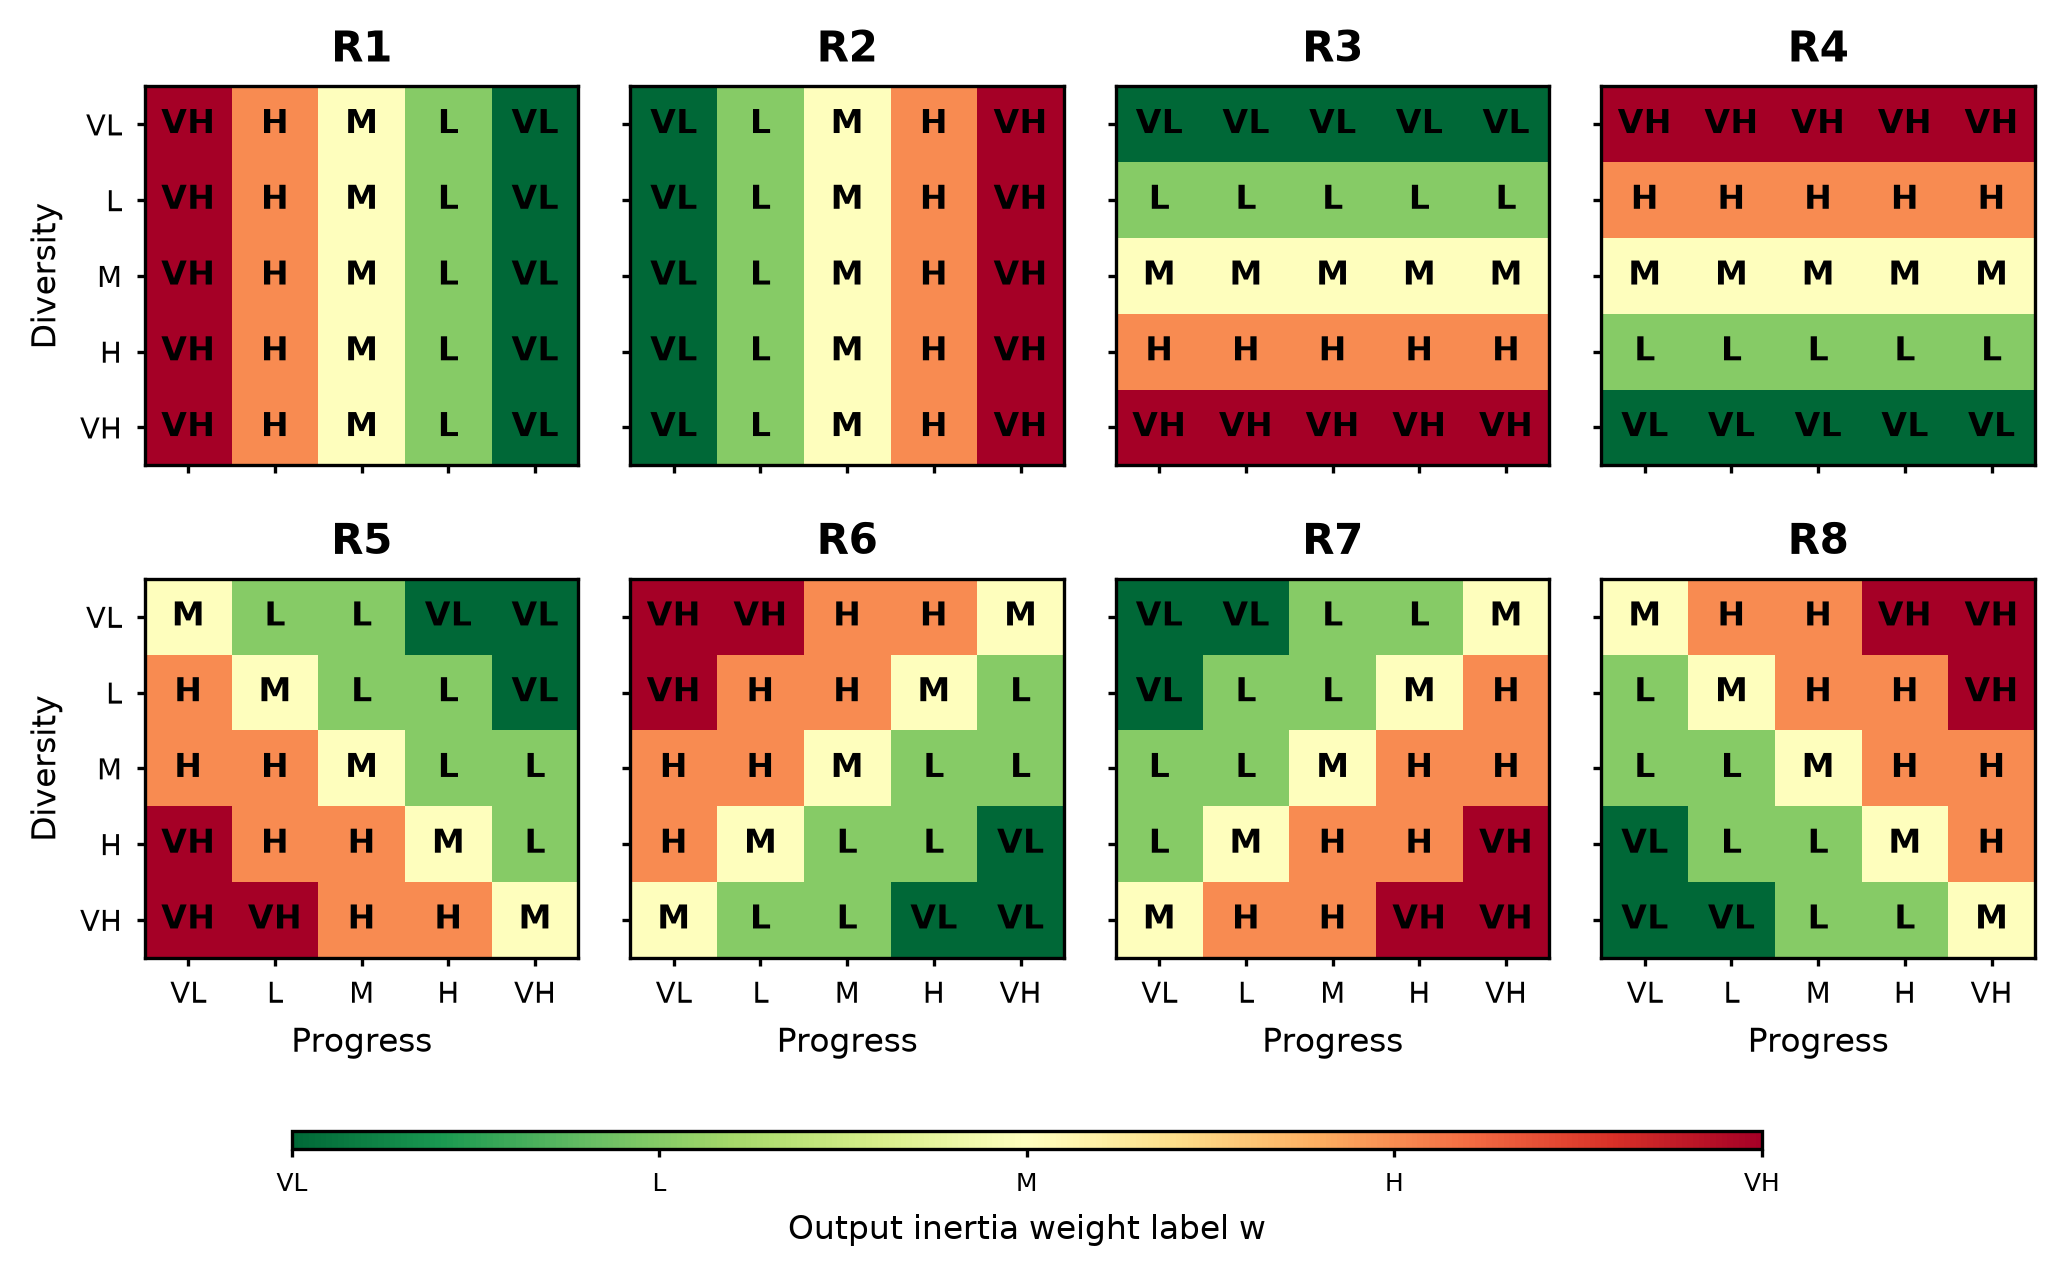
\includegraphics[width=\textwidth,height=0.82\textheight,keepaspectratio]{04_fuzzy_rules_panel_5labels.png}
  \captionof{figure}{Rule-base matrix panel for $n=5$.}
\end{figure}
\begin{figure}[H]\centering
  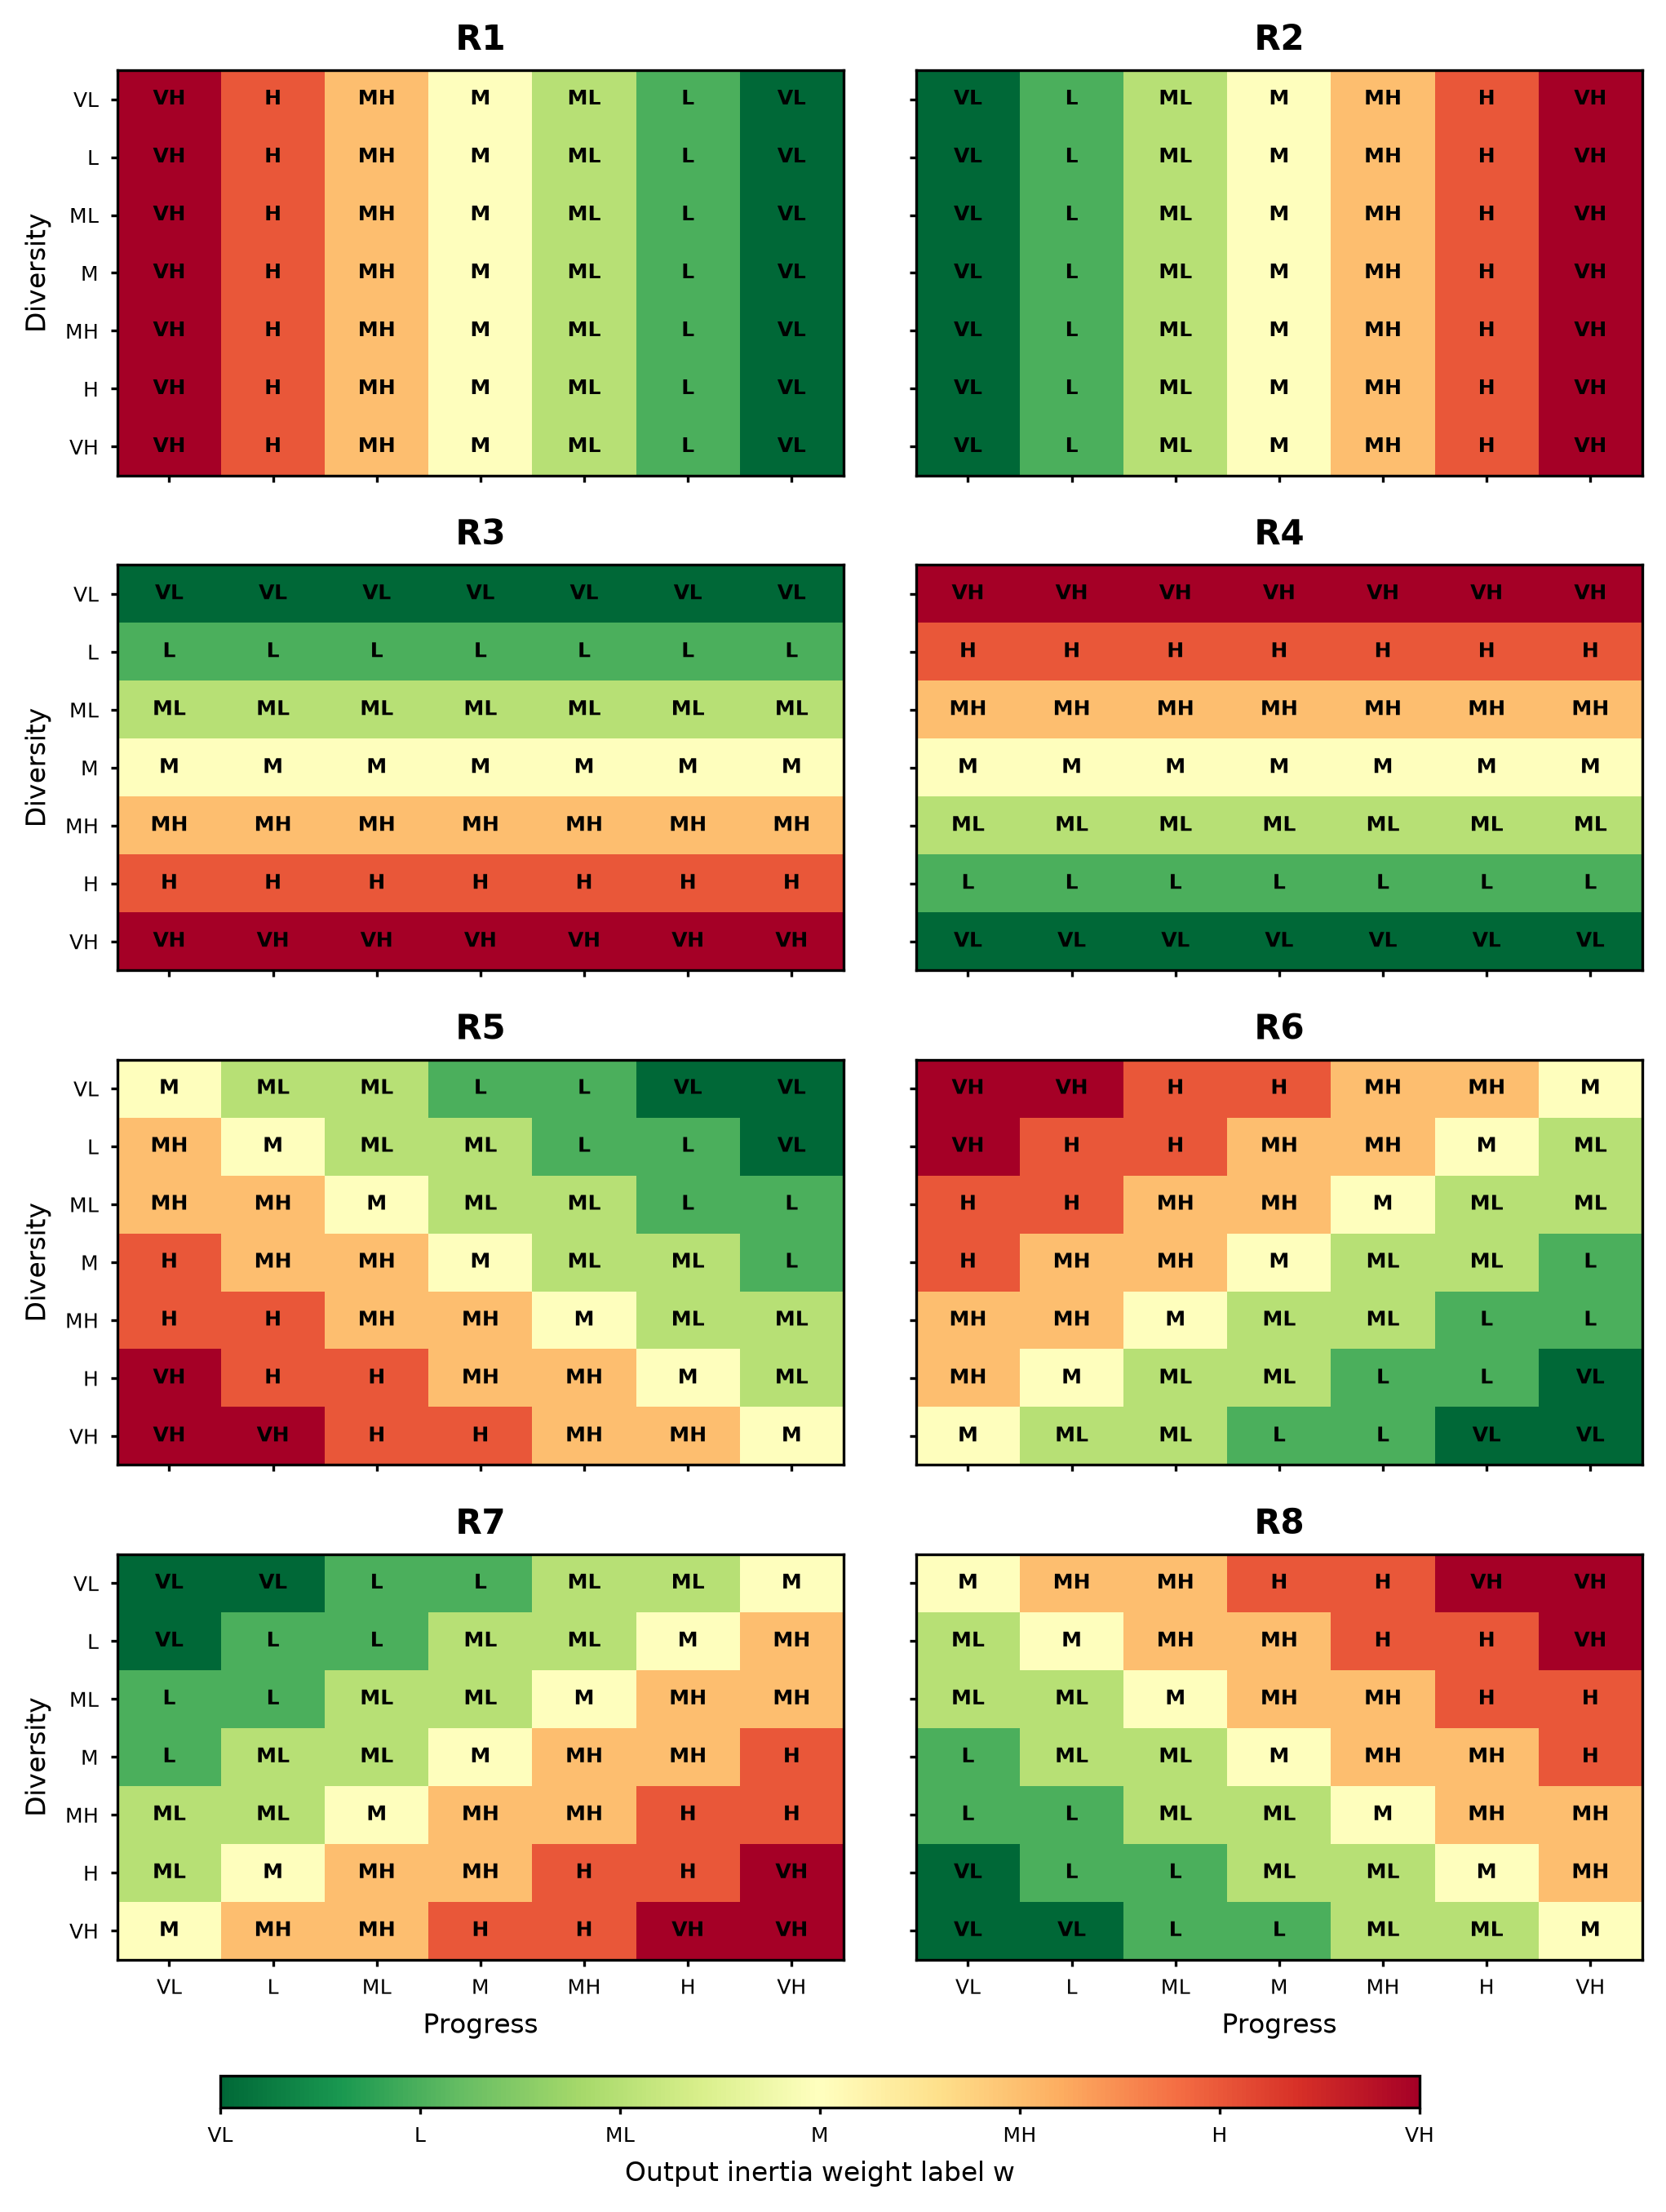
\includegraphics[width=\textwidth,height=0.82\textheight,keepaspectratio]{04_fuzzy_rules_panel_7labels.png}
  \captionof{figure}{Rule-base matrix panel for $n=7$.}
\end{figure}
\begin{figure}[H]\centering
  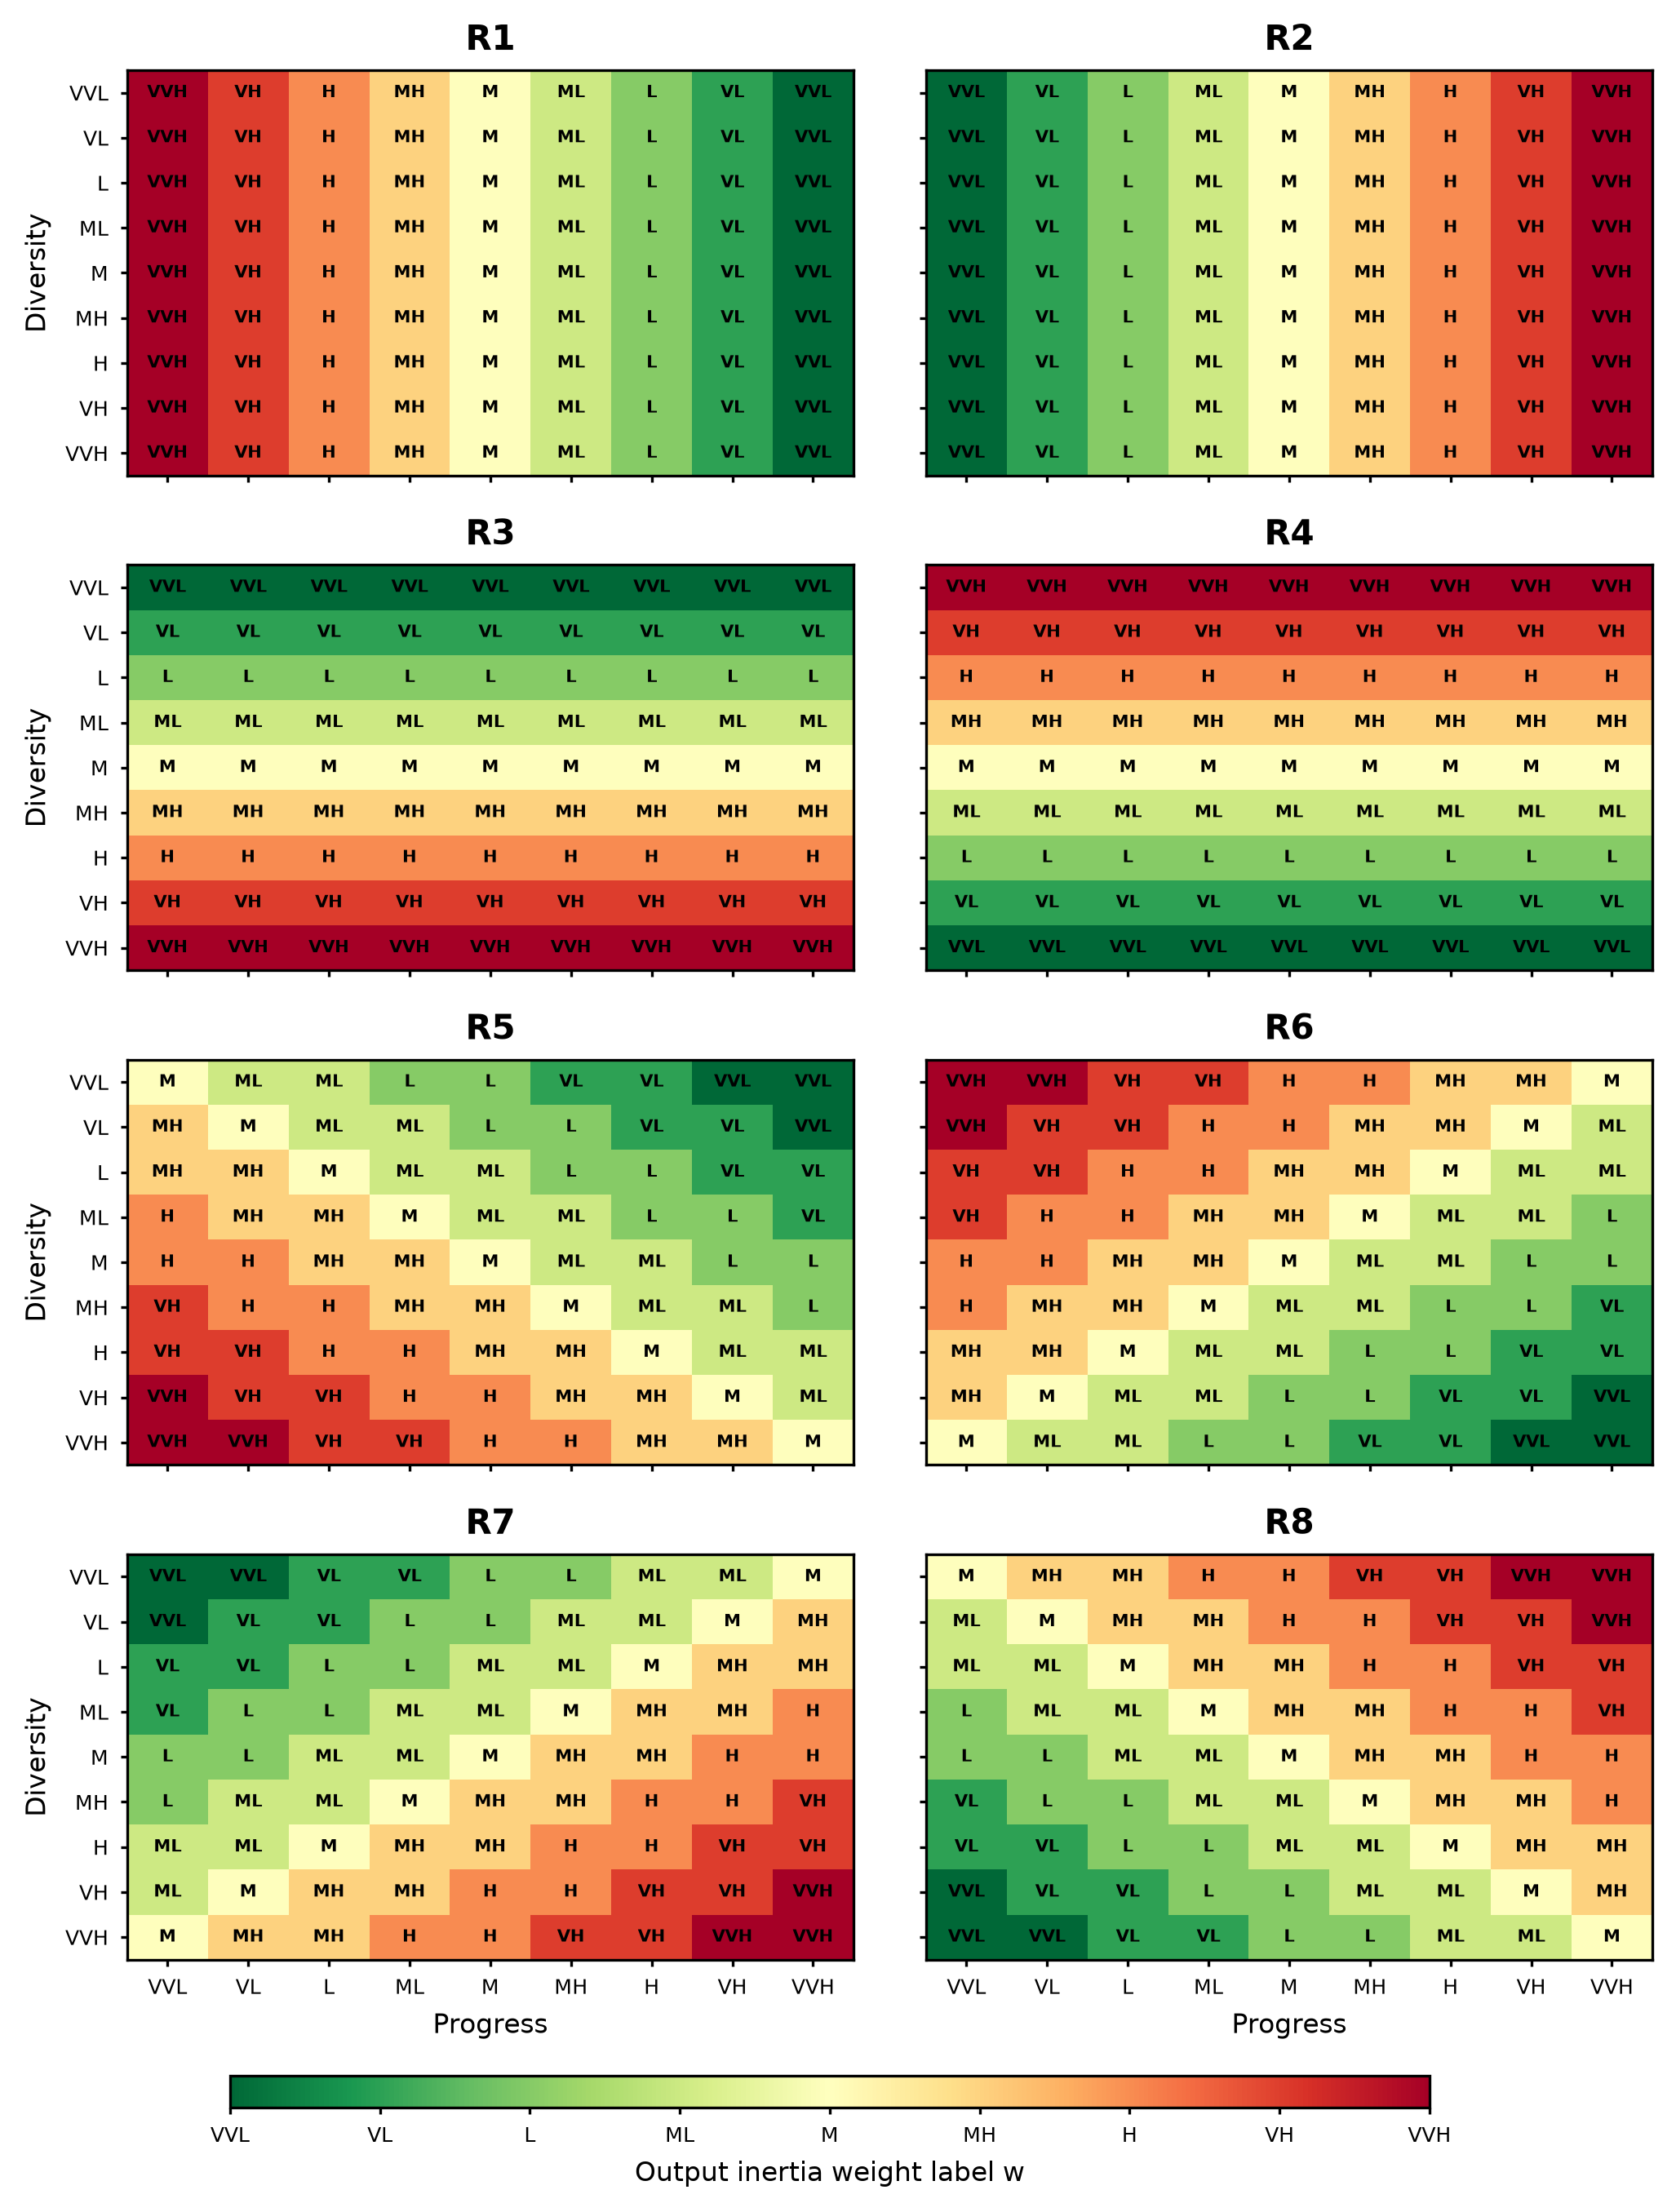
\includegraphics[width=\textwidth,height=0.82\textheight,keepaspectratio]{04_fuzzy_rules_panel_9labels.png}
  \captionof{figure}{Rule-base matrix panel for $n=9$.}
\end{figure}

\subsection{Control surfaces}
Each panel contains the eight rule-induced surfaces for the indicated granularity. Diversity and progress vary over $[0,1]^2$; the output is the defuzzified inertia weight.
\begin{figure}[H]\centering
  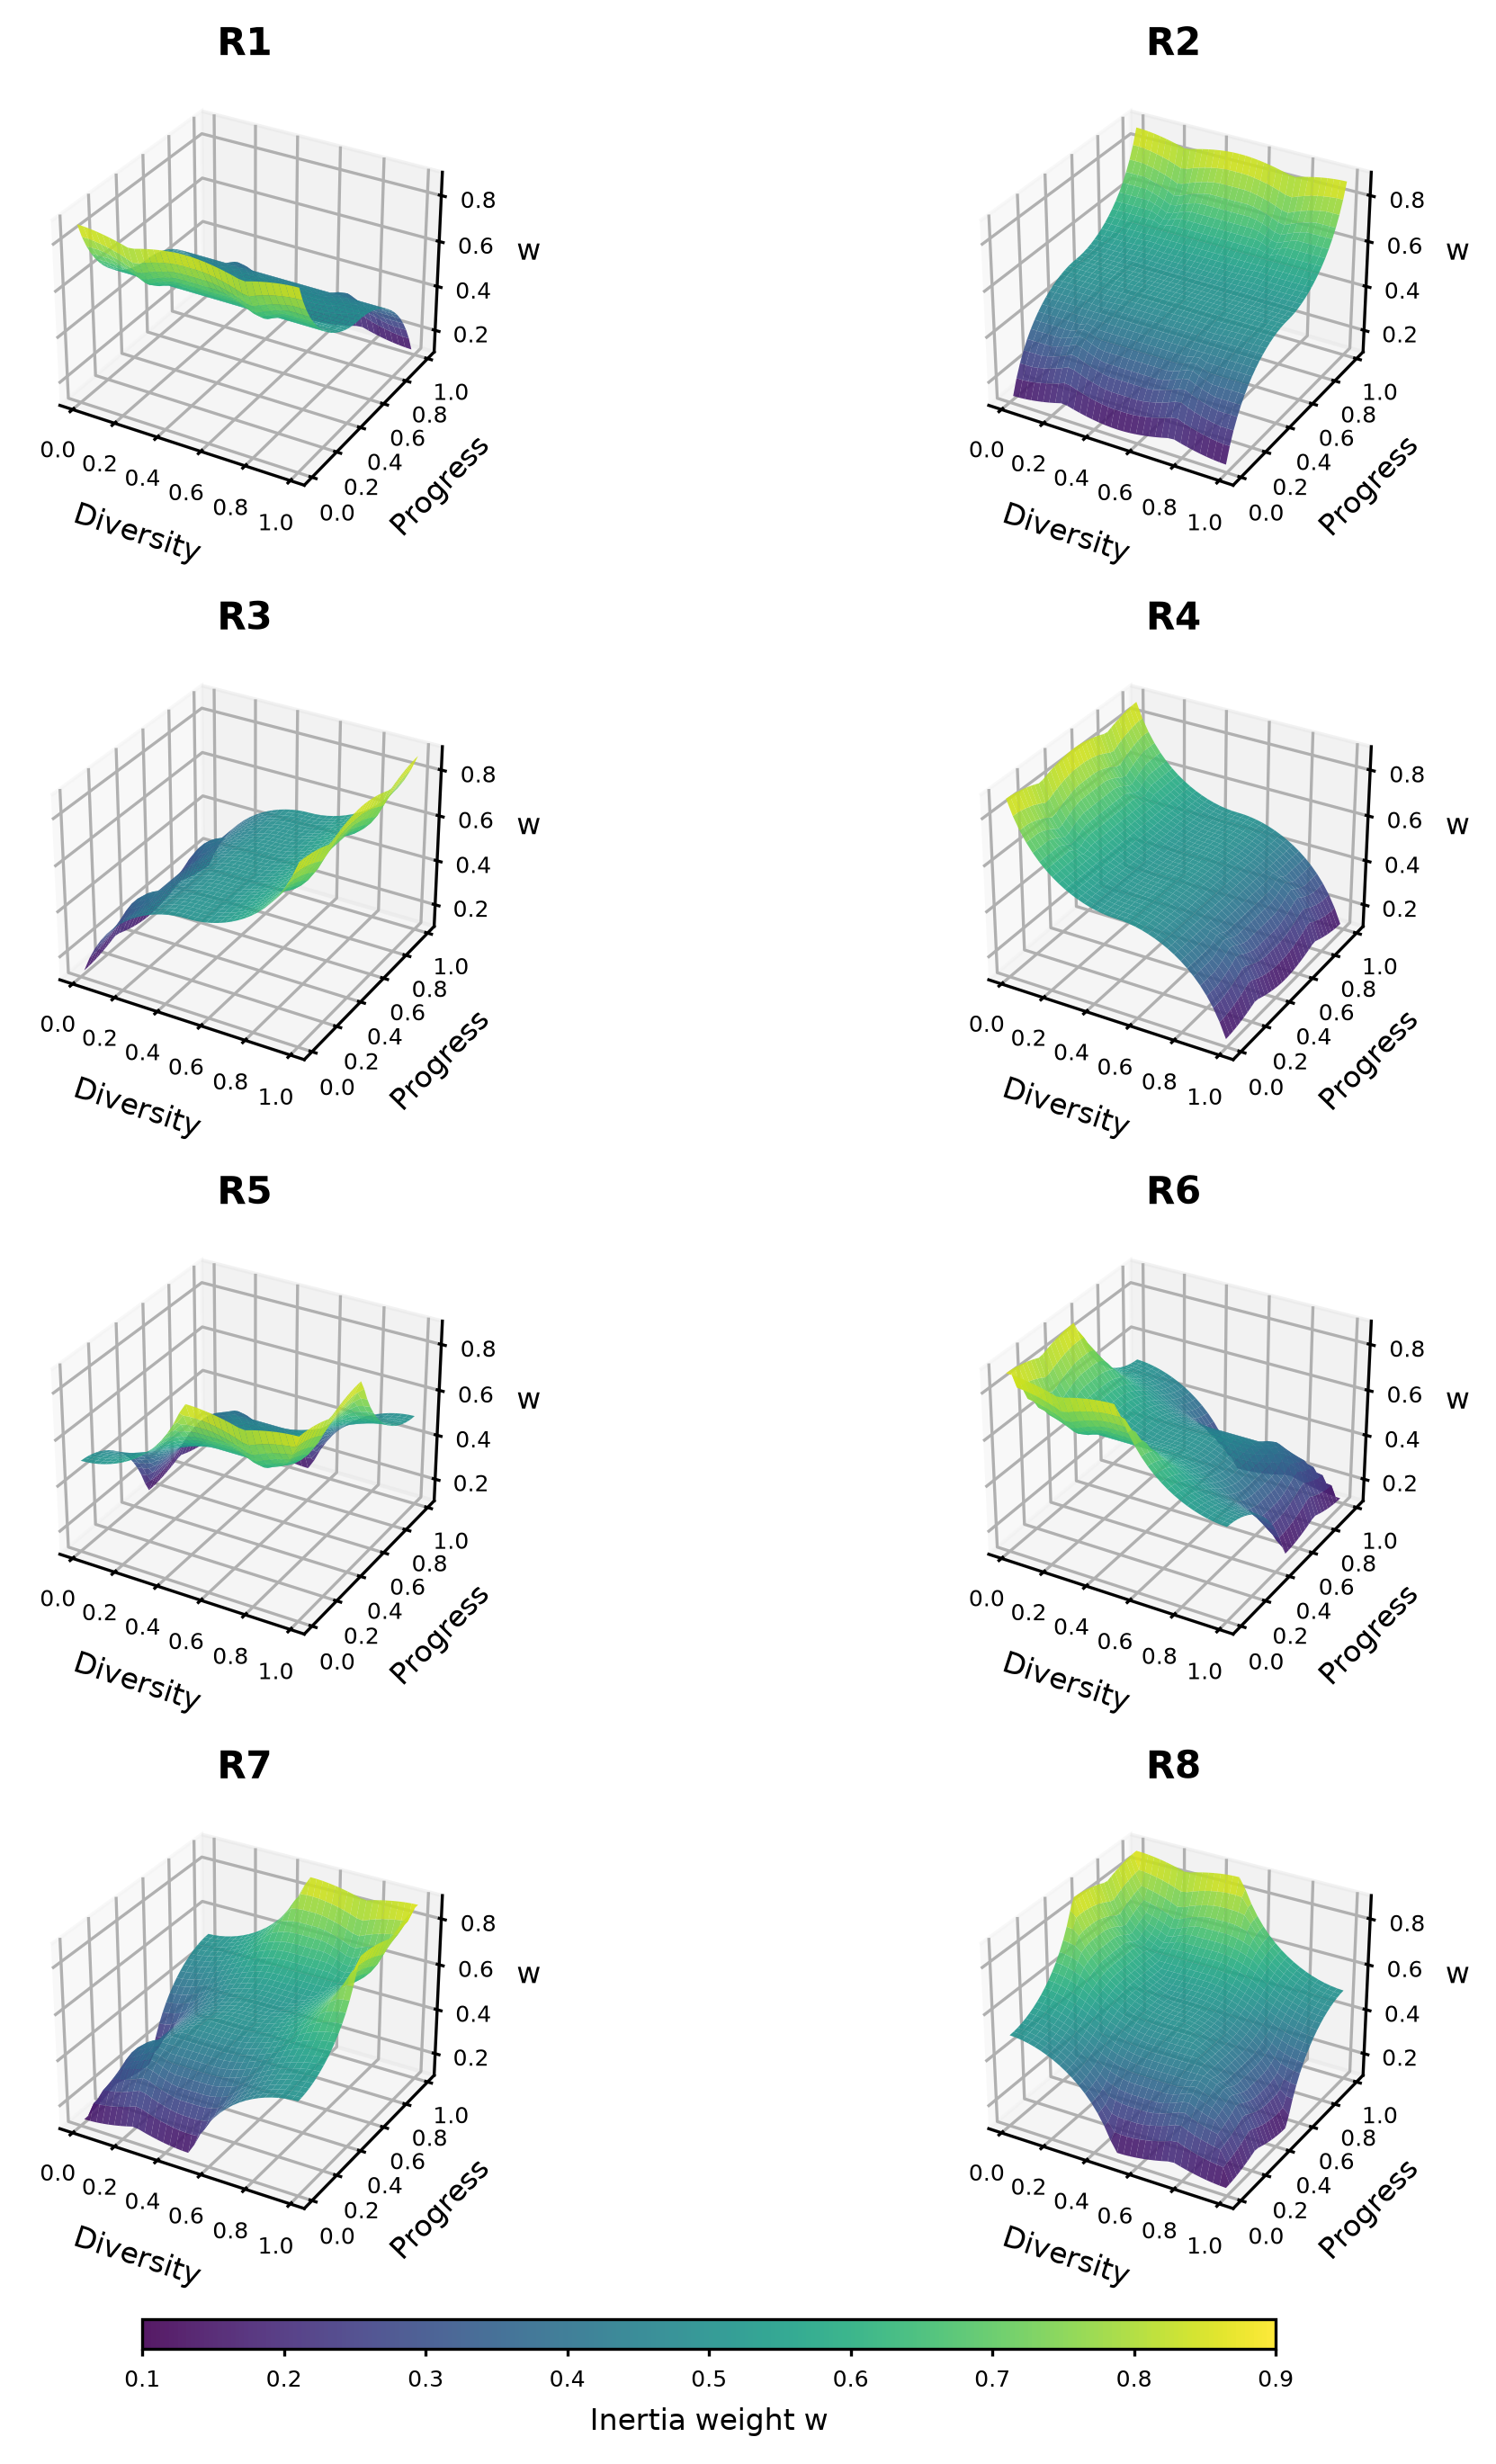
\includegraphics[width=\textwidth,height=0.82\textheight,keepaspectratio]{11_3d_surface_panel_3labels_I1.png}
  \captionof{figure}{Control surfaces for R1--R8 at $n=3$.}
\end{figure}
\begin{figure}[H]\centering
  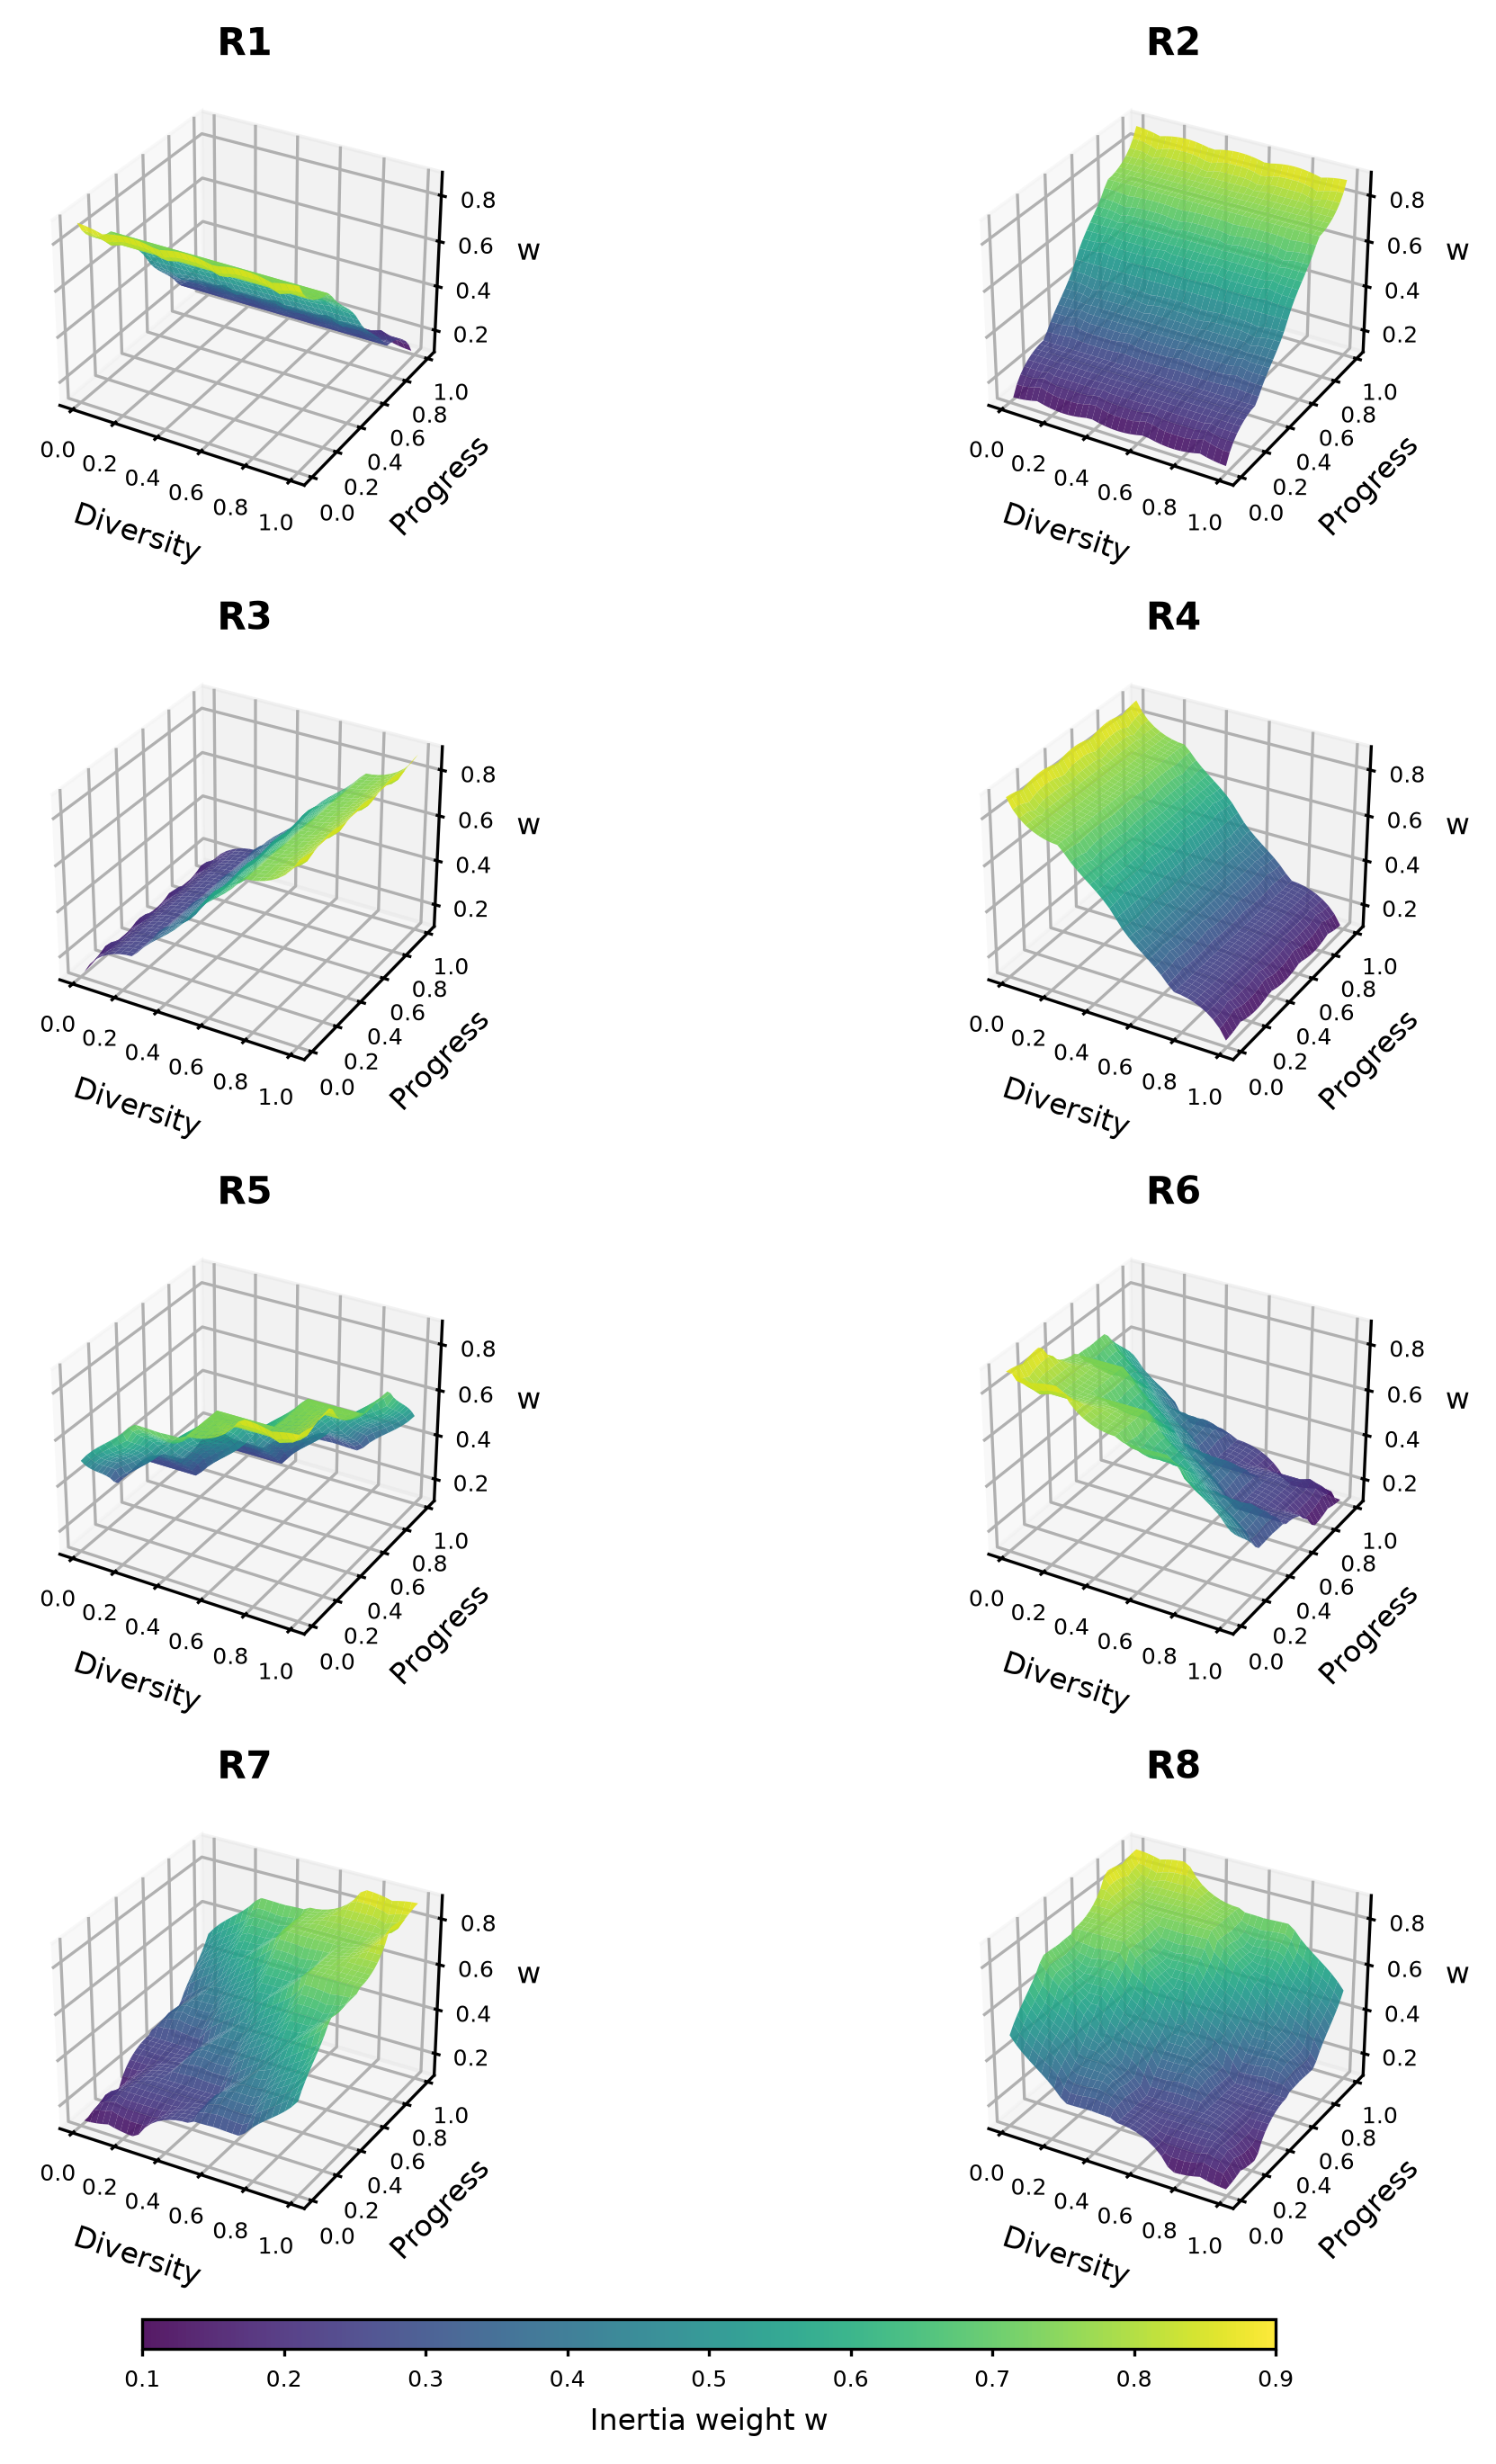
\includegraphics[width=\textwidth,height=0.82\textheight,keepaspectratio]{11_3d_surface_panel_5labels_I1.png}
  \captionof{figure}{Control surfaces for R1--R8 at $n=5$.}
\end{figure}
\begin{figure}[H]\centering
  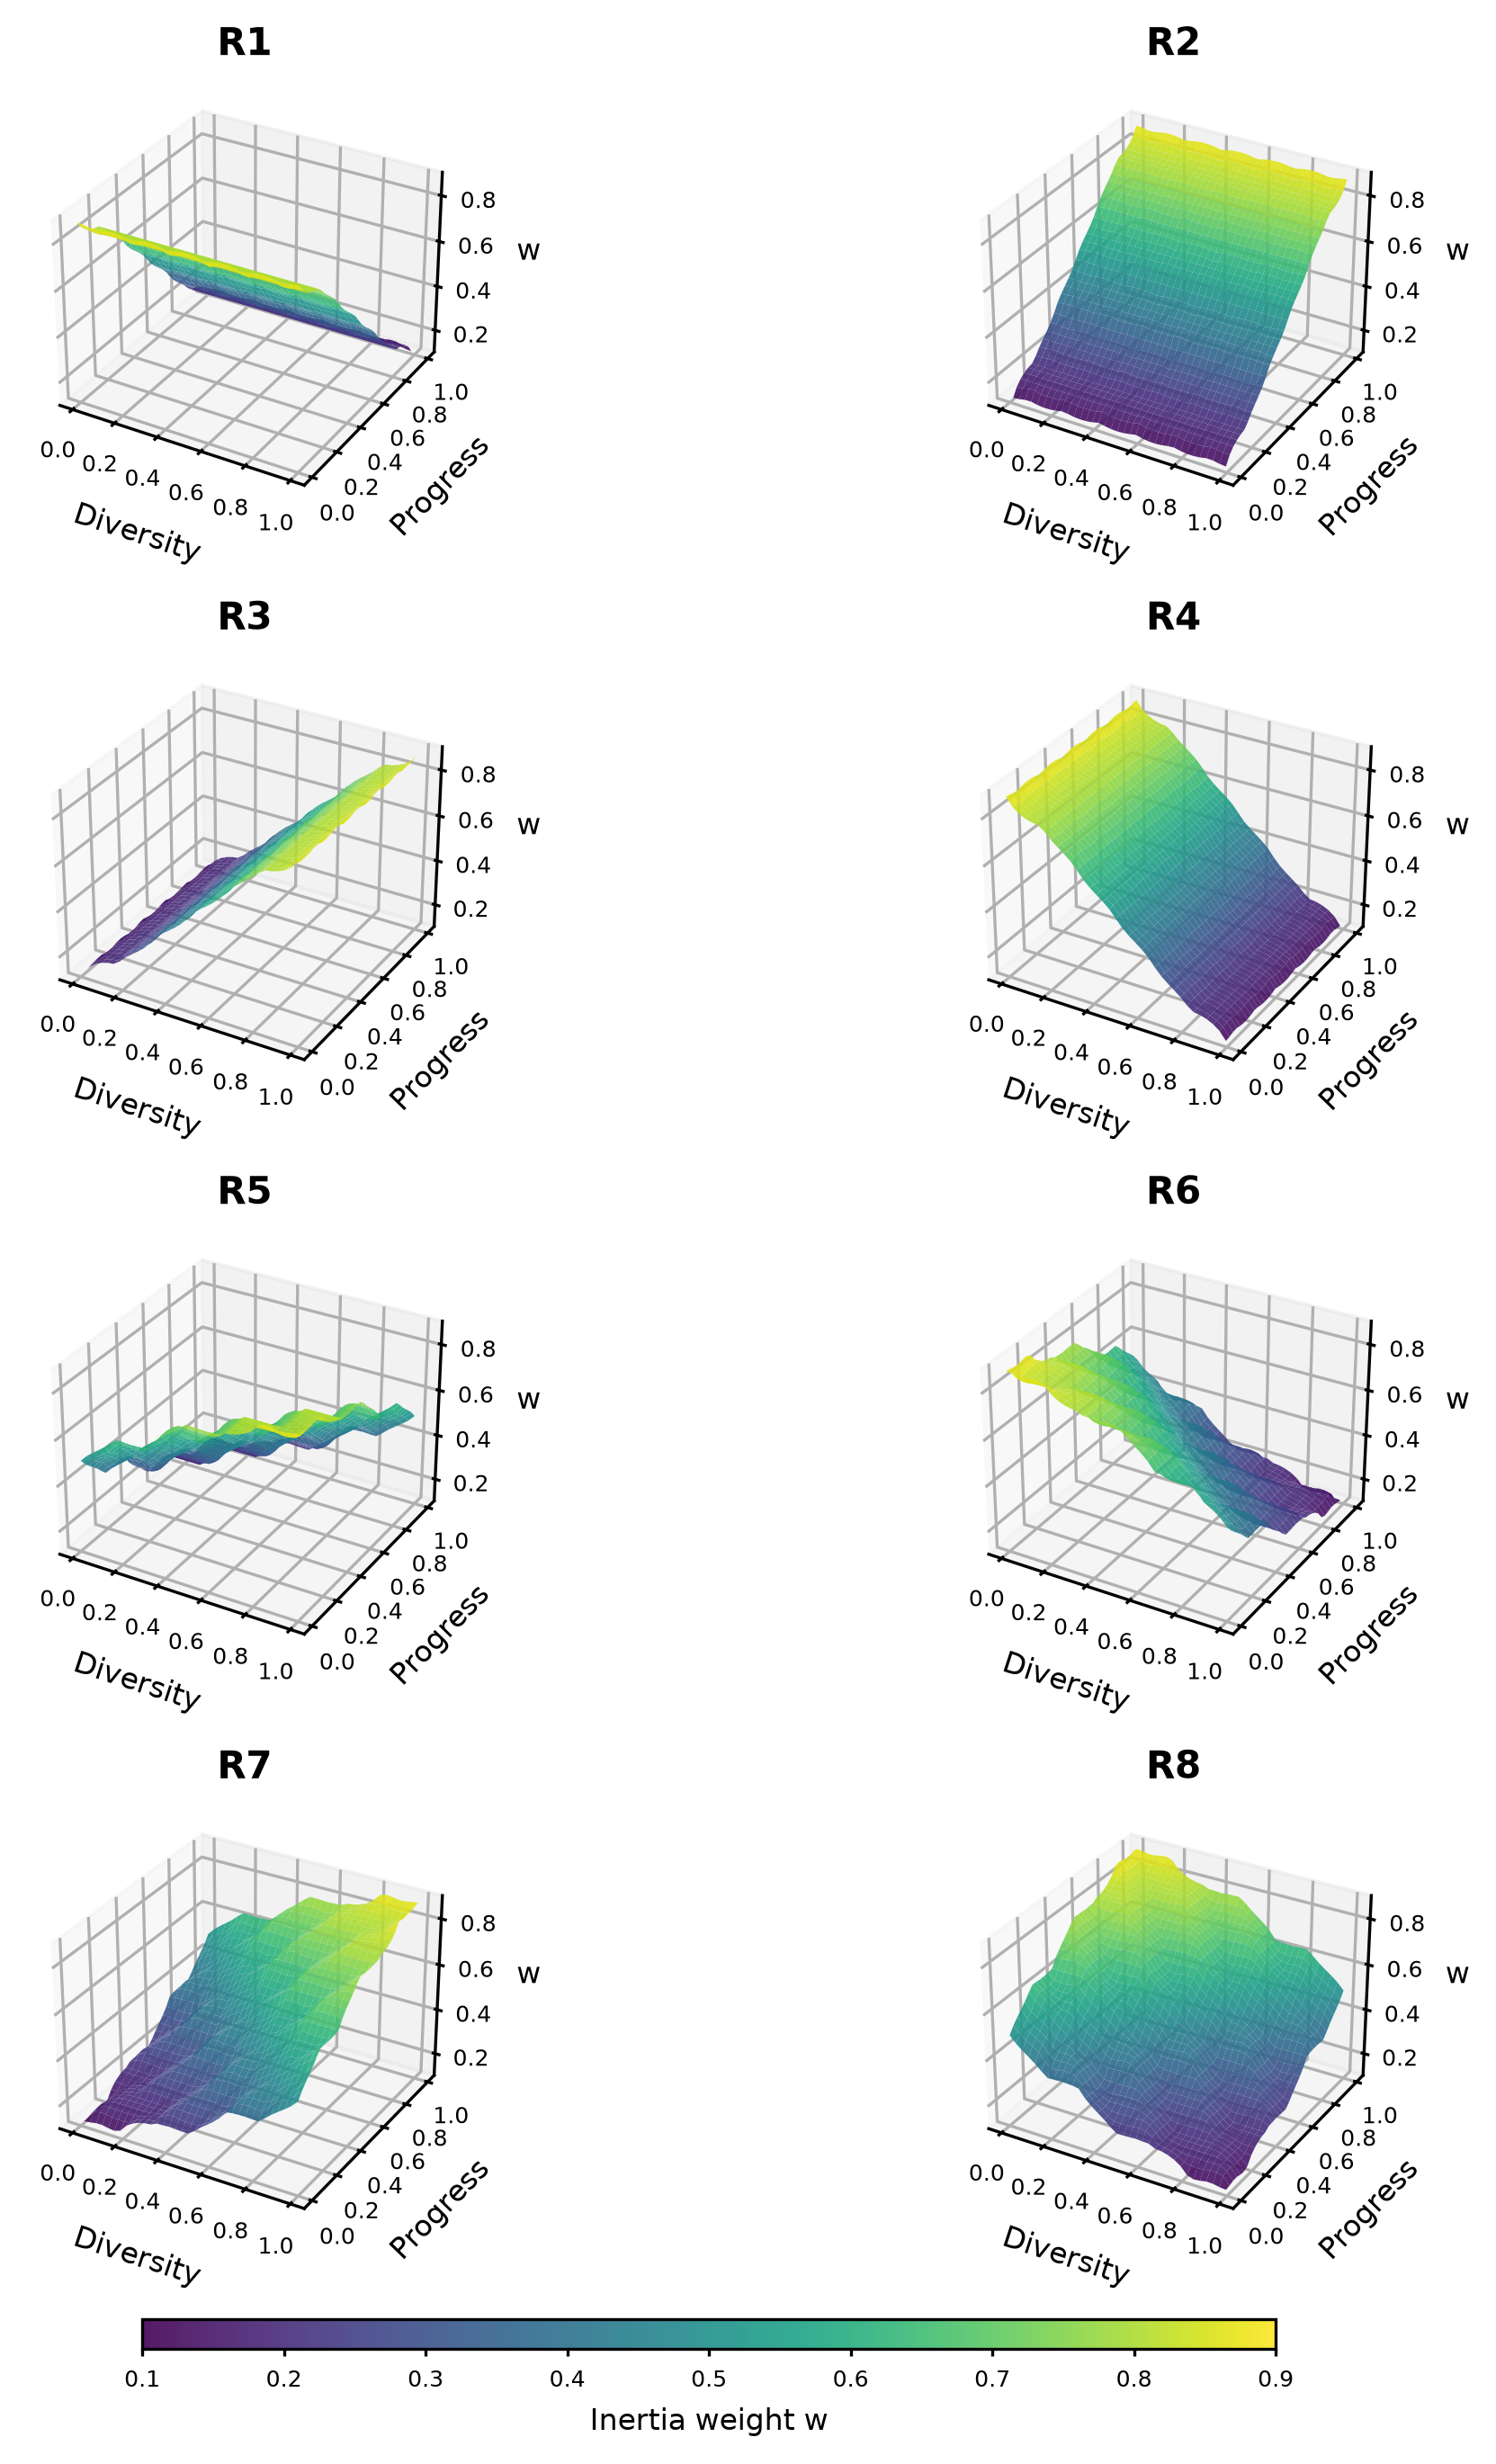
\includegraphics[width=\textwidth,height=0.82\textheight,keepaspectratio]{11_3d_surface_panel_7labels_I1.png}
  \captionof{figure}{Control surfaces for R1--R8 at $n=7$.}
\end{figure}
\begin{figure}[H]\centering
  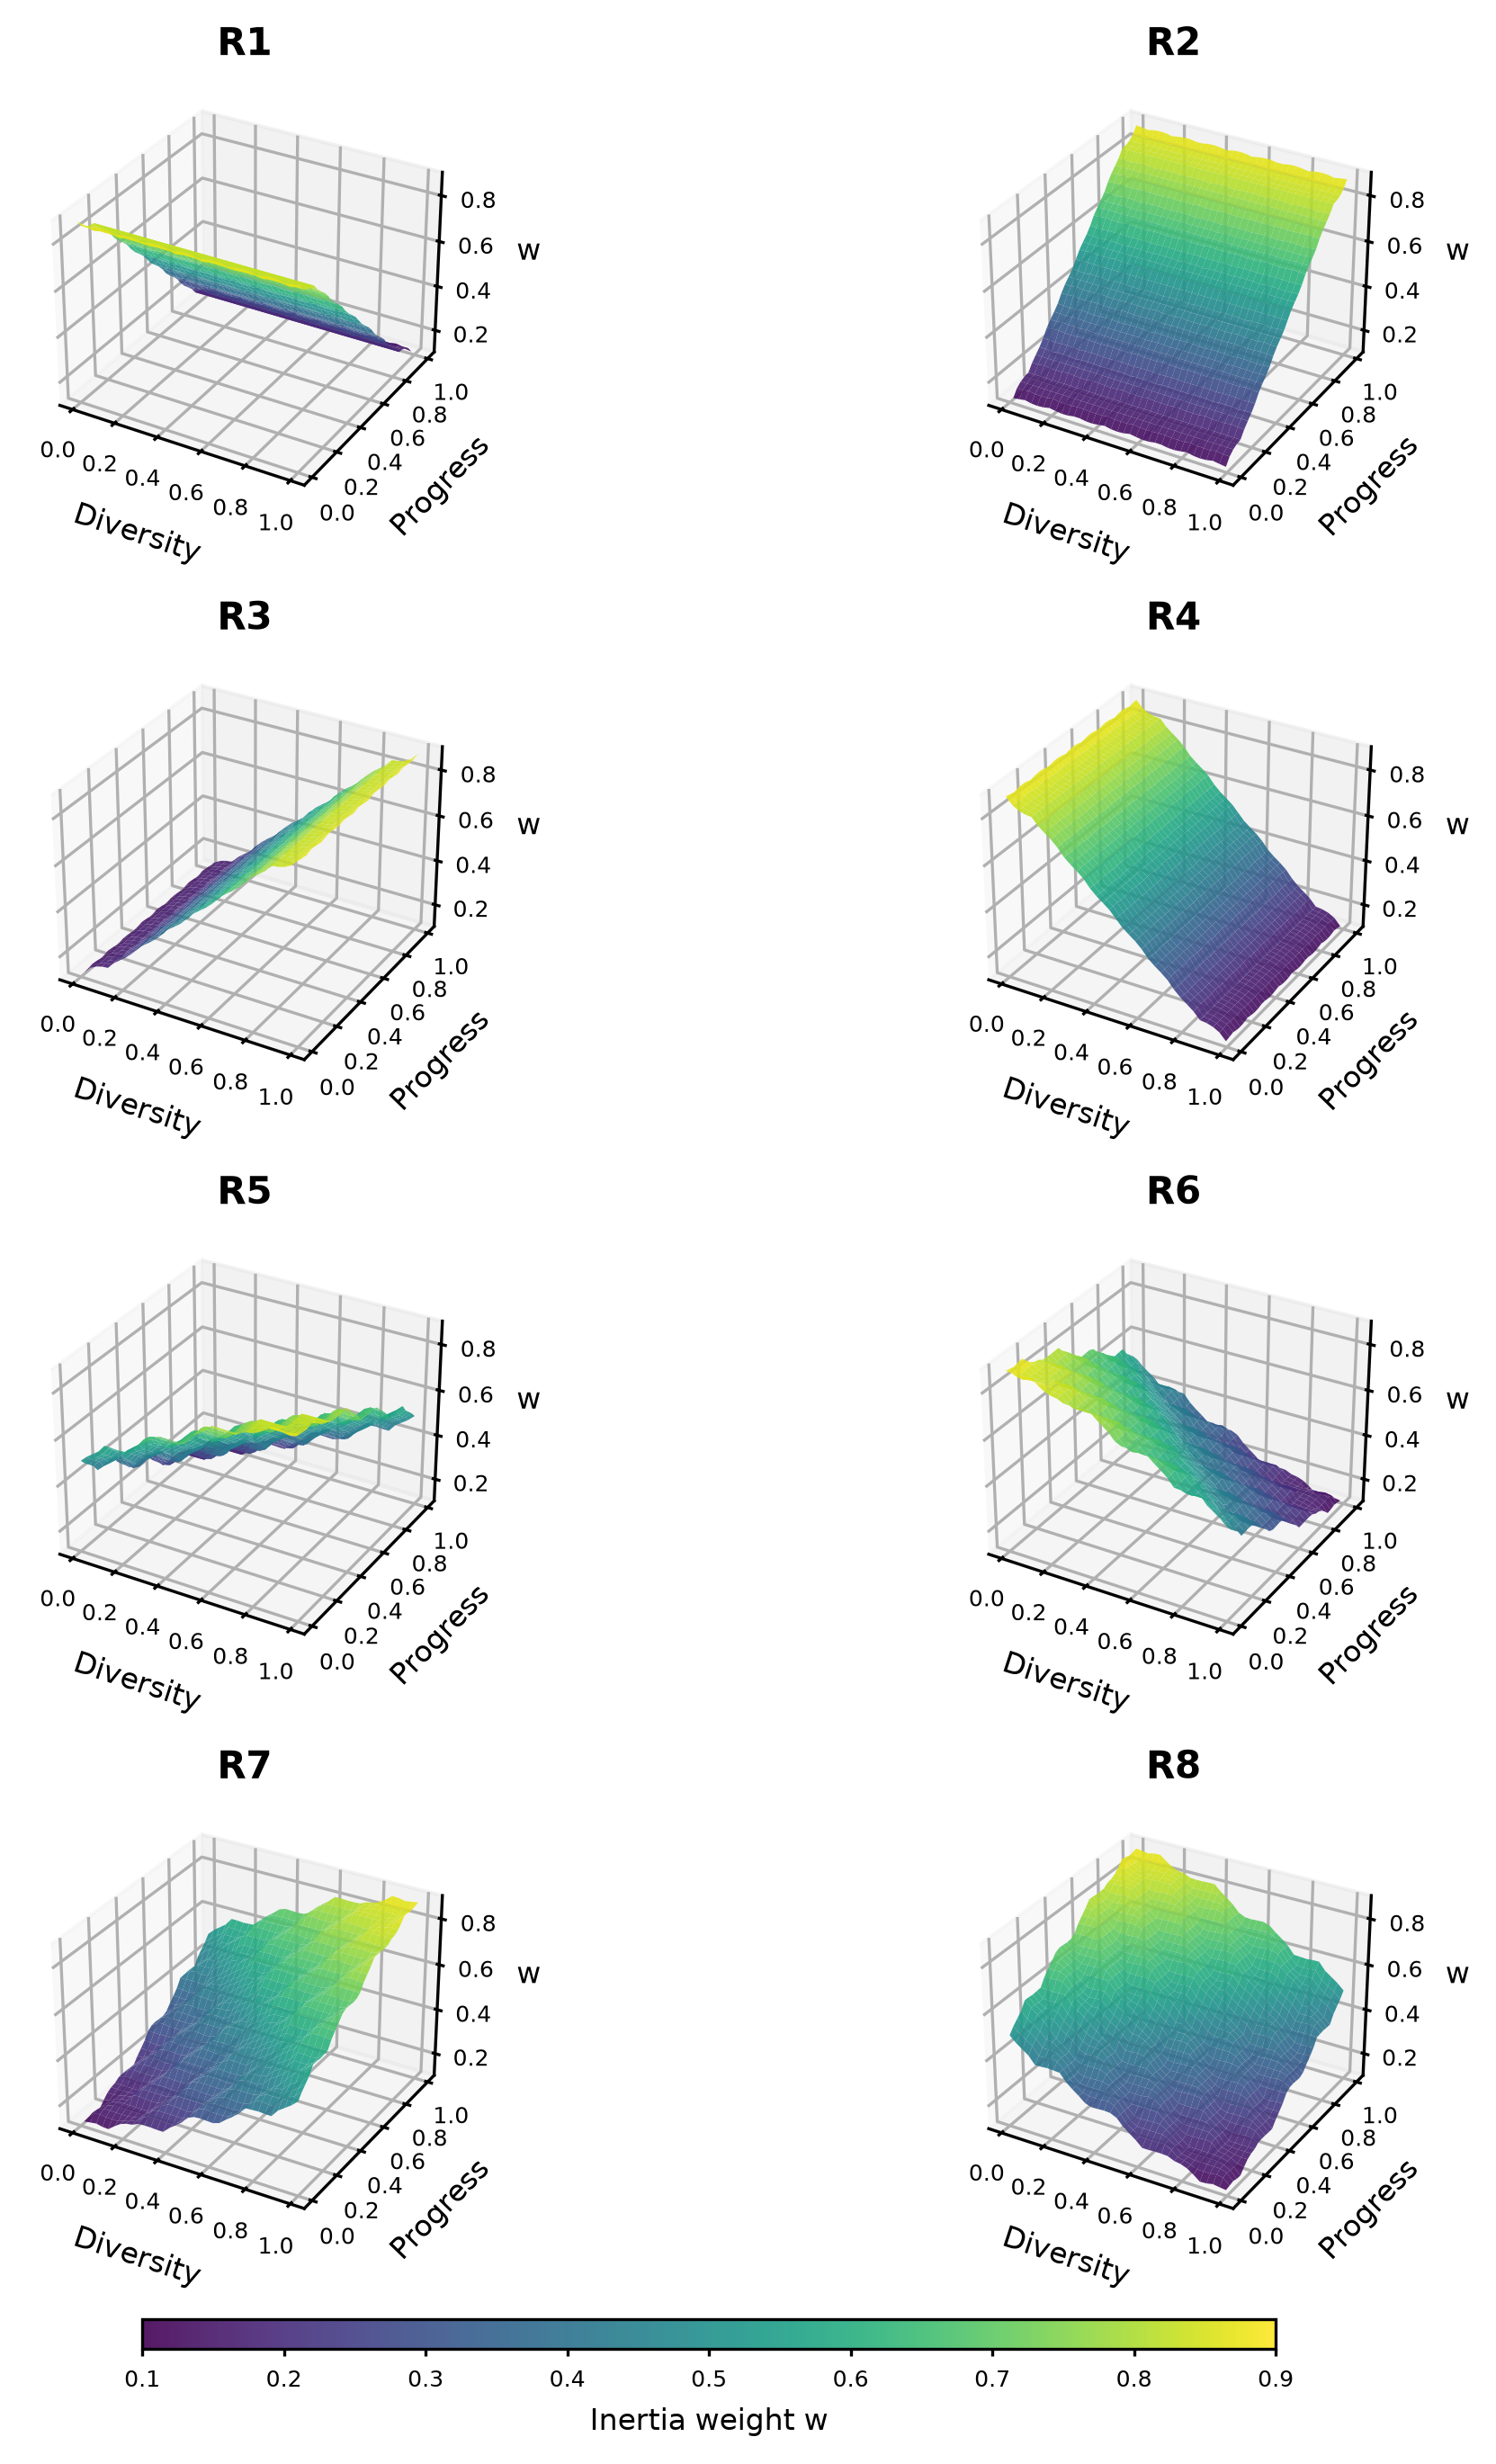
\includegraphics[width=\textwidth,height=0.82\textheight,keepaspectratio]{11_3d_surface_panel_9labels_I1.png}
  \captionof{figure}{Control surfaces for R1--R8 at $n=9$.}
\end{figure}

\section{Complete function-level results}

Table rows correspond to 62 function--dimension instances. Ranks use median normalized gap over all 33 configurations. Each $p$-value is from a two-sided Mann--Whitney $U$ test on independent samples and is Bonferroni-adjusted across the 1,984 RQ4 comparisons. Since fitness is minimized, $A_{12}>0.5$ favours the listed FCS configuration.

\begin{table}[H]
\centering
\footnotesize
\caption{Per-instance FCS--PSO results (part 1 of 3). Ranks use median normalized gap across 33 configurations.}
\label{tab:function_level_full_1}
\setlength{\tabcolsep}{3pt}
\begin{tabular}{llcccccccc}
\toprule
\textbf{Instance} & \textbf{Best FCS} & \boldmath$n$ & \textbf{R} & \textbf{PSO rk.} & \textbf{FCS rk.} & \textbf{PSO gap} & \textbf{FCS gap} & \boldmath$p_{\mathrm{Bonf}}$ & \boldmath$A_{12}$ \\
\midrule
F1\_D10 & \texttt{FCS-3-R1} & 3 & R1 & 5 & 1 & $6.3\!\times10^{-37}$ & $1.4\!\times10^{-44}$ & $<10^{-3}$ & 0.96 \\
F1\_D30 & \texttt{FCS-3-R1} & 3 & R1 & 3 & 1 & $7.7\!\times10^{-6}$ & $1.7\!\times10^{-9}$ & $<10^{-3}$ & 0.97 \\
F1\_D50 & \texttt{FCS-3-R1} & 3 & R1 & 3 & 1 & 0.059 & $1.1\!\times10^{-3}$ & $<10^{-3}$ & 0.99 \\
F1\_D100 & \texttt{FCS-3-R1} & 3 & R1 & 2 & 1 & 16.744 & 10.263 & 1.000 & 0.72 \\
F2\_D10 & \texttt{FCS-3-R1} & 3 & R1 & 6 & 1 & $3.5\!\times10^{-18}$ & $7.7\!\times10^{-25}$ & $<10^{-3}$ & 0.98 \\
F2\_D30 & \texttt{FCS-3-R1} & 3 & R1 & 2 & 1 & $4.5\!\times10^{-4}$ & $5.2\!\times10^{-6}$ & $<10^{-3}$ & 0.98 \\
F2\_D50 & \texttt{FCS-3-R1} & 3 & R1 & 2 & 1 & 0.099 & $8\!\times10^{-3}$ & $<10^{-3}$ & 0.98 \\
F2\_D100 & \texttt{FCS-3-R1} & 3 & R1 & 2 & 1 & 2.357 & 1.375 & $<10^{-3}$ & 0.94 \\
F3\_D10 & \texttt{FCS-5-R5} & 5 & R5 & 9 & 1 & $8.3\!\times10^{-11}$ & $2.8\!\times10^{-15}$ & $<10^{-3}$ & 0.93 \\
F3\_D30 & \texttt{FCS-7-R5} & 7 & R5 & 3 & 1 & 41.57 & 37.246 & 1.000 & 0.58 \\
F3\_D50 & \texttt{FCS-5-R7} & 5 & R7 & 13 & 1 & 1692.014 & 1247.305 & 1.000 & 0.65 \\
F3\_D100 & \texttt{FCS-9-R7} & 9 & R7 & 18 & 1 & $2\!\times10^{4}$ & $1.4\!\times10^{4}$ & 0.027 & 0.82 \\
F4\_D10 & \texttt{FCS-9-R5} & 9 & R5 & 5 & 1 & $1.4\!\times10^{-8}$ & $3.2\!\times10^{-11}$ & $<10^{-3}$ & 0.90 \\
F4\_D30 & \texttt{FCS-9-R1} & 9 & R1 & 6 & 1 & 1.379 & 1.281 & 1.000 & 0.56 \\
F4\_D50 & \texttt{FCS-5-R1} & 5 & R1 & 3 & 1 & 4.347 & 4.234 & 1.000 & 0.56 \\
F4\_D100 & \texttt{FCS-5-R5} & 5 & R5 & 1 & 2 & 14.314 & 14.356 & 1.000 & 0.50 \\
F5\_D10 & \texttt{FCS-3-R1} & 3 & R1 & 5 & 1 & 4.768 & 4.197 & 0.215 & 0.79 \\
F5\_D30 & \texttt{FCS-3-R1} & 3 & R1 & 4 & 1 & 29.198 & 27.947 & 1.000 & 0.50 \\
F5\_D50 & \texttt{FCS-3-R1} & 3 & R1 & 2 & 1 & 150.43 & 116.51 & 1.000 & 0.61 \\
F5\_D100 & \texttt{FCS-3-R1} & 3 & R1 & 2 & 1 & 955.011 & 814.72 & 1.000 & 0.67 \\
F6\_D10 & \texttt{FCS-3-R1} & 3 & R1 & 4 & 1 & $2.8\!\times10^{-32}$ & 0 & 0.006 & 0.82 \\
\bottomrule
\end{tabular}
\par\smallskip
{\raggedright\footnotesize
$p_{\mathrm{Bonf}}$ is the Bonferroni-adjusted two-sided independent-sample Mann--Whitney $U$ $p$-value across 1,984 RQ4 tests. $A_{12}>0.5$ favours the listed FCS because lower fitness is better. Parentheses report configurations sharing the best median-gap rank.\par}
\end{table}
\begin{table}[H]
\centering
\footnotesize
\caption{Per-instance FCS--PSO results (part 2 of 3). Ranks use median normalized gap across 33 configurations.}
\label{tab:function_level_full_2}
\setlength{\tabcolsep}{3pt}
\begin{tabular}{llcccccccc}
\toprule
\textbf{Instance} & \textbf{Best FCS} & \boldmath$n$ & \textbf{R} & \textbf{PSO rk.} & \textbf{FCS rk.} & \textbf{PSO gap} & \textbf{FCS gap} & \boldmath$p_{\mathrm{Bonf}}$ & \boldmath$A_{12}$ \\
\midrule
F6\_D30 & \texttt{FCS-3-R1} & 3 & R1 & 2 & 1 & $2.4\!\times10^{-6}$ & $1.9\!\times10^{-9}$ & $<10^{-3}$ & 0.99 \\
F6\_D50 & \texttt{FCS-3-R1} & 3 & R1 & 2 & 1 & 0.046 & $1.1\!\times10^{-3}$ & $<10^{-3}$ & 0.97 \\
F6\_D100 & \texttt{FCS-3-R1} & 3 & R1 & 2 & 1 & 22.053 & 7.284 & $<10^{-3}$ & 0.93 \\
F7\_D10 & \texttt{FCS-7-R6} & 7 & R6 & 8 & 1 & $1.3\!\times10^{-3}$ & $1\!\times10^{-3}$ & 1.000 & 0.56 \\
F7\_D30 & \texttt{FCS-5-R1} & 5 & R1 & 1 & 2 & $9\!\times10^{-3}$ & $9.1\!\times10^{-3}$ & 1.000 & 0.52 \\
F7\_D50 & \texttt{FCS-3-R1} & 3 & R1 & 2 & 1 & 0.028 & 0.027 & 1.000 & 0.53 \\
F7\_D100 & \texttt{FCS-5-R1} & 5 & R1 & 4 & 1 & 0.142 & 0.132 & 1.000 & 0.55 \\
F8\_D10 & \texttt{FCS-9-R8} & 9 & R8 & 6 & 1 & 0.415 & 0.396 & 1.000 & 0.56 \\
F8\_D30 & \texttt{FCS-7-R3} & 7 & R3 & 12 & 1 & 0.495 & 0.465 & 1.000 & 0.55 \\
F8\_D50 & \texttt{FCS-3-R1} & 3 & R1 & 1 & 2 & 0.483 & 0.491 & 1.000 & 0.43 \\
F8\_D100 & \texttt{FCS-5-R6} & 5 & R6 & 1 & 2 & 0.502 & 0.503 & 1.000 & 0.54 \\
F9\_D10 & \texttt{FCS-5-R2} & 5 & R2 & 11 & 1 & 10.945 & 8.955 & 1.000 & 0.59 \\
F9\_D30 & \texttt{FCS-5-R5} & 5 & R5 & 7 & 1 & 35.818 & 31.853 & 1.000 & 0.56 \\
F9\_D50 & \texttt{FCS-3-R5} & 3 & R5 & 14 & 1 & 67.66 & 55.771 & 1.000 & 0.68 \\
F9\_D100 & \texttt{FCS-7-R5} & 7 & R5 & 4 & 1 & 132.303 & 122.623 & 1.000 & 0.61 \\
F10\_D10 & \texttt{FCS-3-R1} (6 tied) & 3 & R1 & 4 & 4 & $4\!\times10^{-15}$ & $4\!\times10^{-15}$ & 1.000 & 0.45 \\
F10\_D30 & \texttt{FCS-3-R1} & 3 & R1 & 2 & 1 & $6.6\!\times10^{-4}$ & $1.5\!\times10^{-5}$ & $<10^{-3}$ & 0.93 \\
F10\_D50 & \texttt{FCS-3-R1} & 3 & R1 & 4 & 1 & 0.522 & 0.019 & 0.094 & 0.80 \\
F10\_D100 & \texttt{FCS-3-R1} & 3 & R1 & 3 & 1 & 2.192 & 1.966 & 1.000 & 0.74 \\
F11\_D10 & \texttt{FCS-9-R1} & 9 & R1 & 10 & 1 & 0.091 & 0.069 & 1.000 & 0.64 \\
F11\_D30 & \texttt{FCS-7-R1} & 7 & R1 & 5 & 1 & $7.5\!\times10^{-3}$ & $1.4\!\times10^{-3}$ & 1.000 & 0.54 \\
\bottomrule
\end{tabular}
\par\smallskip
{\raggedright\footnotesize
$p_{\mathrm{Bonf}}$ is the Bonferroni-adjusted two-sided independent-sample Mann--Whitney $U$ $p$-value across 1,984 RQ4 tests. $A_{12}>0.5$ favours the listed FCS because lower fitness is better. Parentheses report configurations sharing the best median-gap rank.\par}
\end{table}
\begin{table}[H]
\centering
\footnotesize
\caption{Per-instance FCS--PSO results (part 3 of 3). Ranks use median normalized gap across 33 configurations.}
\label{tab:function_level_full_3}
\setlength{\tabcolsep}{3pt}
\begin{tabular}{llcccccccc}
\toprule
\textbf{Instance} & \textbf{Best FCS} & \boldmath$n$ & \textbf{R} & \textbf{PSO rk.} & \textbf{FCS rk.} & \textbf{PSO gap} & \textbf{FCS gap} & \boldmath$p_{\mathrm{Bonf}}$ & \boldmath$A_{12}$ \\
\midrule
F11\_D50 & \texttt{FCS-3-R1} & 3 & R1 & 3 & 1 & 0.064 & 0.012 & $<10^{-3}$ & 0.91 \\
F11\_D100 & \texttt{FCS-3-R1} & 3 & R1 & 2 & 1 & 1.168 & 1.042 & 0.004 & 0.85 \\
F12\_D10 & \texttt{FCS-3-R1} & 3 & R1 & 2 & 1 & $4.8\!\times10^{-32}$ & $4.7\!\times10^{-32}$ & 0.284 & 0.77 \\
F12\_D30 & \texttt{FCS-3-R1} & 3 & R1 & 2 & 1 & $1.2\!\times10^{-8}$ & $2.1\!\times10^{-11}$ & 0.065 & 0.81 \\
F12\_D50 & \texttt{FCS-7-R1} & 7 & R1 & 1 & 2 & $4.1\!\times10^{-4}$ & $4.9\!\times10^{-4}$ & 1.000 & 0.49 \\
F12\_D100 & \texttt{FCS-5-R1} & 5 & R1 & 3 & 1 & 2.769 & 2.313 & 1.000 & 0.67 \\
F13\_D10 & \texttt{FCS-3-R1} & 3 & R1 & 3 & 1 & $1.8\!\times10^{-32}$ & $1.3\!\times10^{-32}$ & 0.126 & 0.76 \\
F13\_D30 & \texttt{FCS-3-R1} & 3 & R1 & 2 & 1 & $2.4\!\times10^{-6}$ & $9.4\!\times10^{-9}$ & 1.000 & 0.65 \\
F13\_D50 & \texttt{FCS-3-R1} & 3 & R1 & 3 & 1 & 0.025 & $8.9\!\times10^{-3}$ & 0.112 & 0.80 \\
F13\_D100 & \texttt{FCS-3-R1} & 3 & R1 & 3 & 1 & 16.942 & 9.312 & 1.000 & 0.73 \\
F14\_D2 & \texttt{FCS-3-R1} (6 tied) & 3 & R1 & 27 & 3 & 2.968 & 0.992 & 1.000 & 0.58 \\
F15\_D4 & \texttt{FCS-3-R1} & 3 & R1 & 11 & 1 & $7.5\!\times10^{-6}$ & $7.5\!\times10^{-6}$ & 1.000 & 0.75 \\
F16\_D2 & \texttt{FCS-3-R1} (32 tied) & 3 & R1 & 17 & 17 & 0 & 0 & 1.000 & 0.56 \\
F17\_D2 & \texttt{FCS-3-R1} (32 tied) & 3 & R1 & 17 & 17 & 0 & 0 & 1.000 & 0.50 \\
F18\_D2 & \texttt{FCS-3-R1} (28 tied) & 3 & R1 & 15 & 15 & 0 & 0 & 1.000 & 0.45 \\
F19\_D3 & \texttt{FCS-3-R1} (32 tied) & 3 & R1 & 17 & 17 & 0 & 0 & 1.000 & 0.56 \\
F20\_D6 & \texttt{FCS-3-R1} (27 tied) & 3 & R1 & 14 & 14 & 0 & 0 & 1.000 & 0.55 \\
F21\_D4 & \texttt{FCS-7-R1} & 7 & R1 & 24 & 1 & 0.736 & 0 & 1.000 & 0.61 \\
F22\_D4 & \texttt{FCS-3-R6} (2 tied) & 3 & R6 & 20 & 1 & 0.642 & 0 & 1.000 & 0.57 \\
F23\_D4 & \texttt{FCS-5-R6} & 5 & R6 & 1 & 2 & 0 & $1.7\!\times10^{-16}$ & 1.000 & 0.34 \\
\bottomrule
\end{tabular}
\par\smallskip
{\raggedright\footnotesize
$p_{\mathrm{Bonf}}$ is the Bonferroni-adjusted two-sided independent-sample Mann--Whitney $U$ $p$-value across 1,984 RQ4 tests. $A_{12}>0.5$ favours the listed FCS because lower fitness is better. Parentheses report configurations sharing the best median-gap rank.\par}
\end{table}


\section{Performance versus run-to-run dispersion}

The 23-page atlas shows one page per benchmark function. Scalable functions include one panel per tested dimension with shared axis limits. Each point gives the mean and standard deviation of normalized gap over 31 runs for one configuration--instance pair. Logarithmic axes display zero at $10^{-12}$. Colour identifies rule-base pattern, marker shape identifies granularity, the star marks PSO, and the open circle marks the selected FCS. Overlapping points denote equal summaries; axis ranges vary by function.

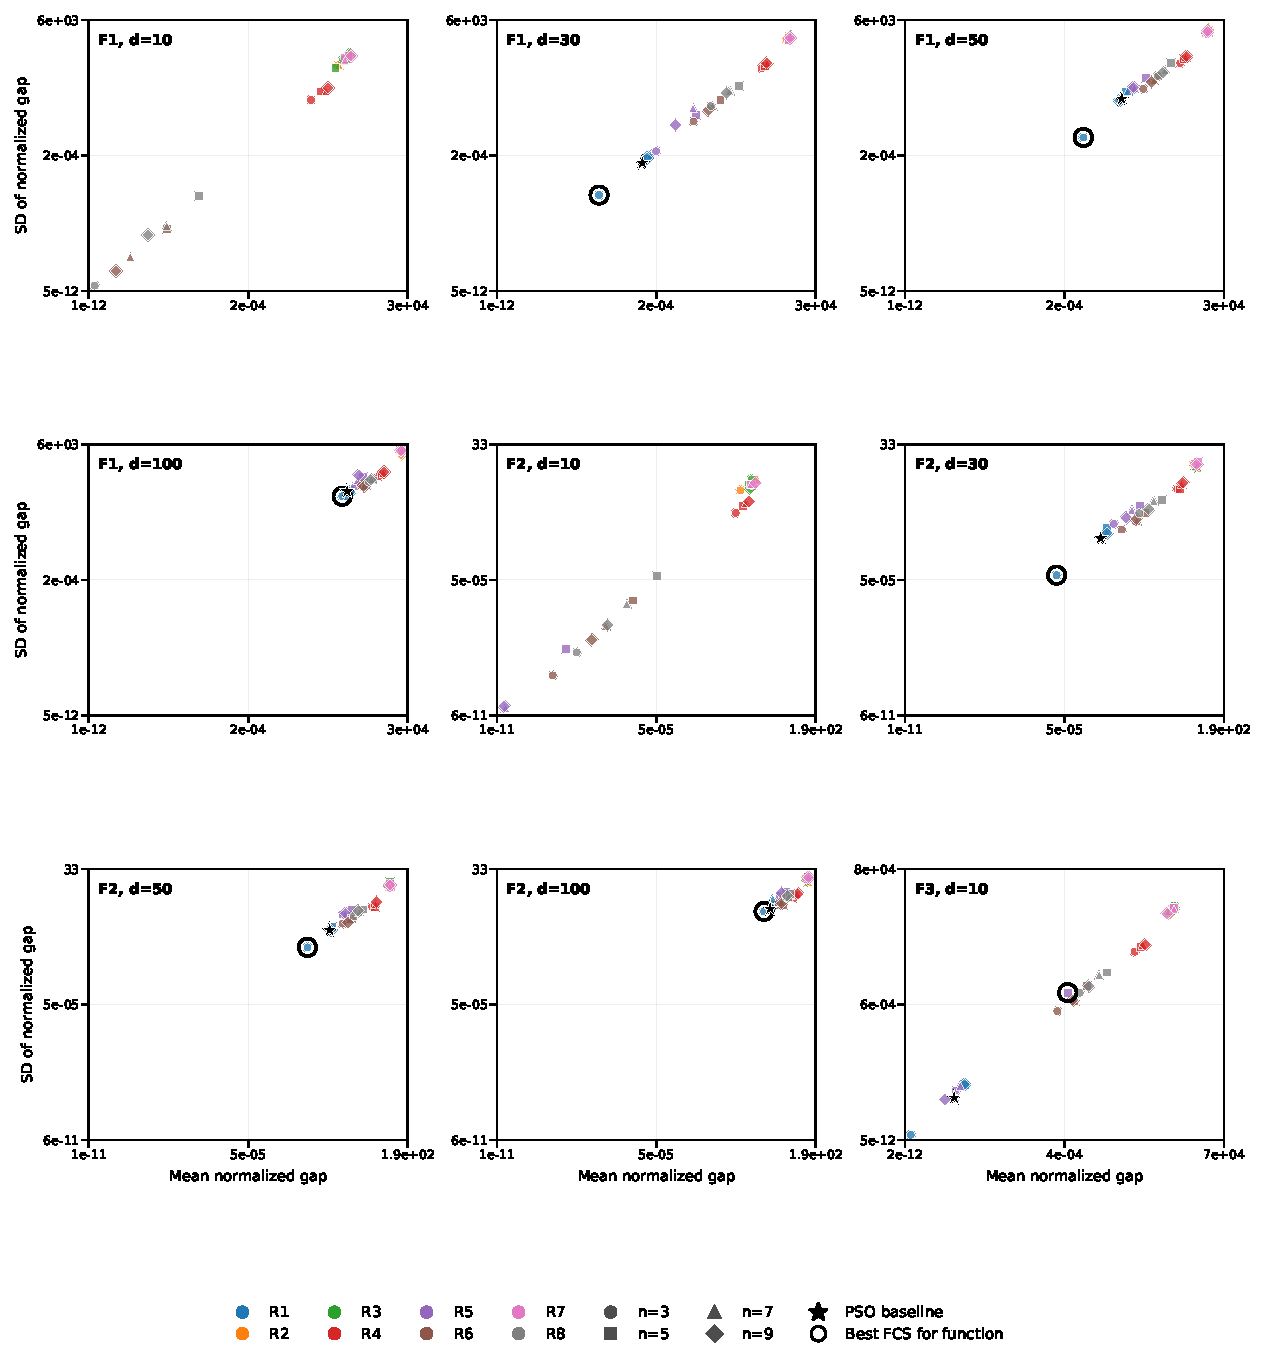
\includepdf[pages=-,scale=0.97,pagecommand={\thispagestyle{plain}}]{SupplementaryData/figures/fig_mean_dispersion_by_function.pdf}

\section{Benchmark-function landscape slices}

Each page pairs a contour with a 3-D view of the same two-dimensional slice. Coordinates use the benchmark bounds; dimensions beyond two are fixed at the bounds midpoint. Elevation and colour show $\log_{10}(1+\max(f(x)-f^*,0))$. F8 uses its dimension-scaled optimum, and F7 shows the expected objective with uniform-noise mean $0.5$.

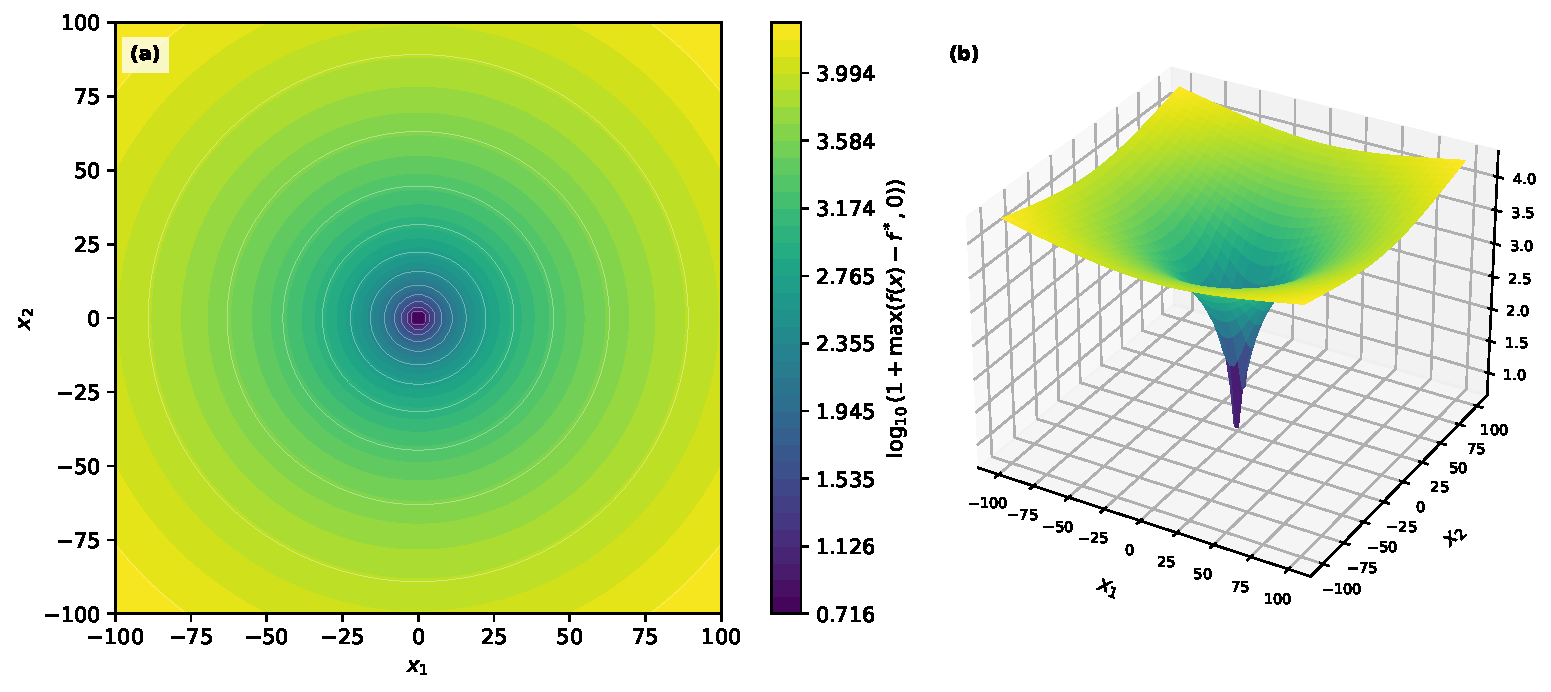
\includepdf[pages=-,pagecommand={\thispagestyle{plain}}]{SupplementaryData/figures/benchmark_landscape_slices.pdf}

\section{Supporting data}

The Supplementary Materials provide consolidated run-level outcomes and machine-readable summaries for the rankings, independent-sample tests, effect sizes, runtime estimates, granularity profiles, and controller trajectories. RQ3 is descriptive and does not estimate a factorial interaction.

\end{document}
